\documentclass[10pt,twocolumn,letterpaper]{article}

\usepackage{cvpr}
\usepackage{times}
\usepackage{epsfig}
\usepackage{graphicx}
\usepackage{amsmath}
\usepackage{amssymb}
\usepackage{dsfont}
\usepackage{enumitem}

%%%%%%%%%%%%%%
% Packages and stuff custom
%%%%%%%%%%%%%%
\usepackage{url}
\usepackage{amsthm}
\usepackage{color}
\usepackage{subcaption}
\captionsetup{compatibility=false}
\usepackage{booktabs}
%\usepackage{hyperref}
% If you comment hyperref and then uncomment it, you should delete
% egpaper.aux before re-running latex.  (Or just hit 'q' on the first latex
% run, let it finish, and you should be clear).
\usepackage[pagebackref=true,breaklinks=true,letterpaper=true,colorlinks,bookmarks=false]{hyperref}

\DeclareMathOperator{\E}{\mathbb{E}}
\DeclareMathOperator{\R}{\mathbb{R}}

\def\figref#1{Fig.~\ref{#1}}
\def\secref#1{\S\ref{#1}}
\def\tabref#1{Table~\ref{#1}}
\def\eqnref#1{Eq.~\ref{#1}}

\newcommand{\ow}[1]{\textbf{\textcolor[rgb]{.1, .1, .8}{OW: #1}}}
\newcommand{\rz}[1]{\textbf{\textcolor[rgb]{.54, .16, .55}{RZ: #1}}}
\newcommand{\todo}[1]{\textbf{\textcolor[rgb]{.8, .1, .1}{#1}}}
\newcommand{\pd}[1]{\textbf{\textcolor[rgb]{1, 0.5, 0}{PD: #1}}}
\newcommand{\eli}[1]{\textbf{\textcolor[rgb]{0.1, 0.6, 0.1}{ES: #1}}}



\newcommand{\addSubFigHalf}[3]{\begin{subfigure}[t]{.45\linewidth}
   \includegraphics[width=\linewidth]{#1}
   \caption{#2}\label{#3}\end{subfigure}
}
\newcommand{\addSubFigThird}[3]{\begin{subfigure}[t]{.31\linewidth}
   \includegraphics[width=\linewidth]{#1}
   \caption{#2}\label{#3}\end{subfigure}
}
\newcommand{\addSubFigTenth}[3]{\begin{subfigure}[t]{.16\linewidth}
   \includegraphics[width=\linewidth]{#1}
   \caption{#2}\label{#3}\end{subfigure}
}
\newcommand{\addSubFigSixth}[2]{\begin{subfigure}[t]{.12\linewidth}
   \includegraphics[width=\linewidth]{#1}
   \label{#2}\end{subfigure}
}
\newcommand{\addSubFigSixthLabel}[3]{\begin{subfigure}[t]{.12\linewidth}
   %\rotatebox{90}{#2}
   \includegraphics[width=\linewidth]{#1}
   \caption{#2}\label{#3}\end{subfigure}
}



\newcommand{\model}[0]{GateGAN}

\DeclareGraphicsExtensions{.pdf,.jpg}

%%%%%%%%%%%%%%%

\graphicspath{ {images/}{syntheticExp/} {final_images/channel_gated/} {final_images/} {paper_images/} }
%%%%%%%%%%%%%%%%


% Include other packages here, before hyperref.

% If you comment hyperref and then uncomment it, you should delete
% egpaper.aux before re-running latex.  (Or just hit 'q' on the first latex
% run, let it finish, and you should be clear).
\usepackage[pagebackref=true,breaklinks=true,letterpaper=true,colorlinks,bookmarks=false]{hyperref}

% \cvprfinalcopy % *** Uncomment this line for the final submission

\def\cvprPaperID{2914} % *** Enter the CVPR Paper ID here
\def\httilde{\mbox{\tt\raisebox{-.5ex}{\symbol{126}}}}

% Pages are numbered in submission mode, and unnumbered in camera-ready
\ifcvprfinal\pagestyle{empty}\fi
\begin{document}

%%%%%%%%% TITLE
\title{GAN-Gate: Gated residual GANs for Class Conditioned Image Generation}

\author{Arnab Ghosh\\
University of Oxford\\
{\tt\small arnab.ghosh@eng.ox.ac.uk}
% For a paper whose authors are all at the same institution,
% omit the following lines up until the closing ``}''.
% Additional authors and addresses can be added with ``\and'',
% just like the second author.
% To save space, use either the email address or home page, not both
\and
Puneet Dokania\\
University of Oxford\\
{\tt\small puneet@robots.ox.ac.uk}
\and
Richard Zhang\\
Adobe Research\\
{\tt\small rizhang@adobe.com}
\and
Oliver Wang\\
Adobe Research\\
{\tt\small owang@adobe.com}
\and
Philip Torr\\
University of Oxford\\
{\tt\small philip.torr@eng.ox.ac.uk}
\and
Eli Shechtman\\
Adobe Research\\
{\tt\small elishe@adobe.com}
}

%\maketitle
%\thispagestyle{empty}


\twocolumn[{%
\renewcommand\twocolumn[1][]{#1}%
\maketitle
\begin{center}
    \centering
    % 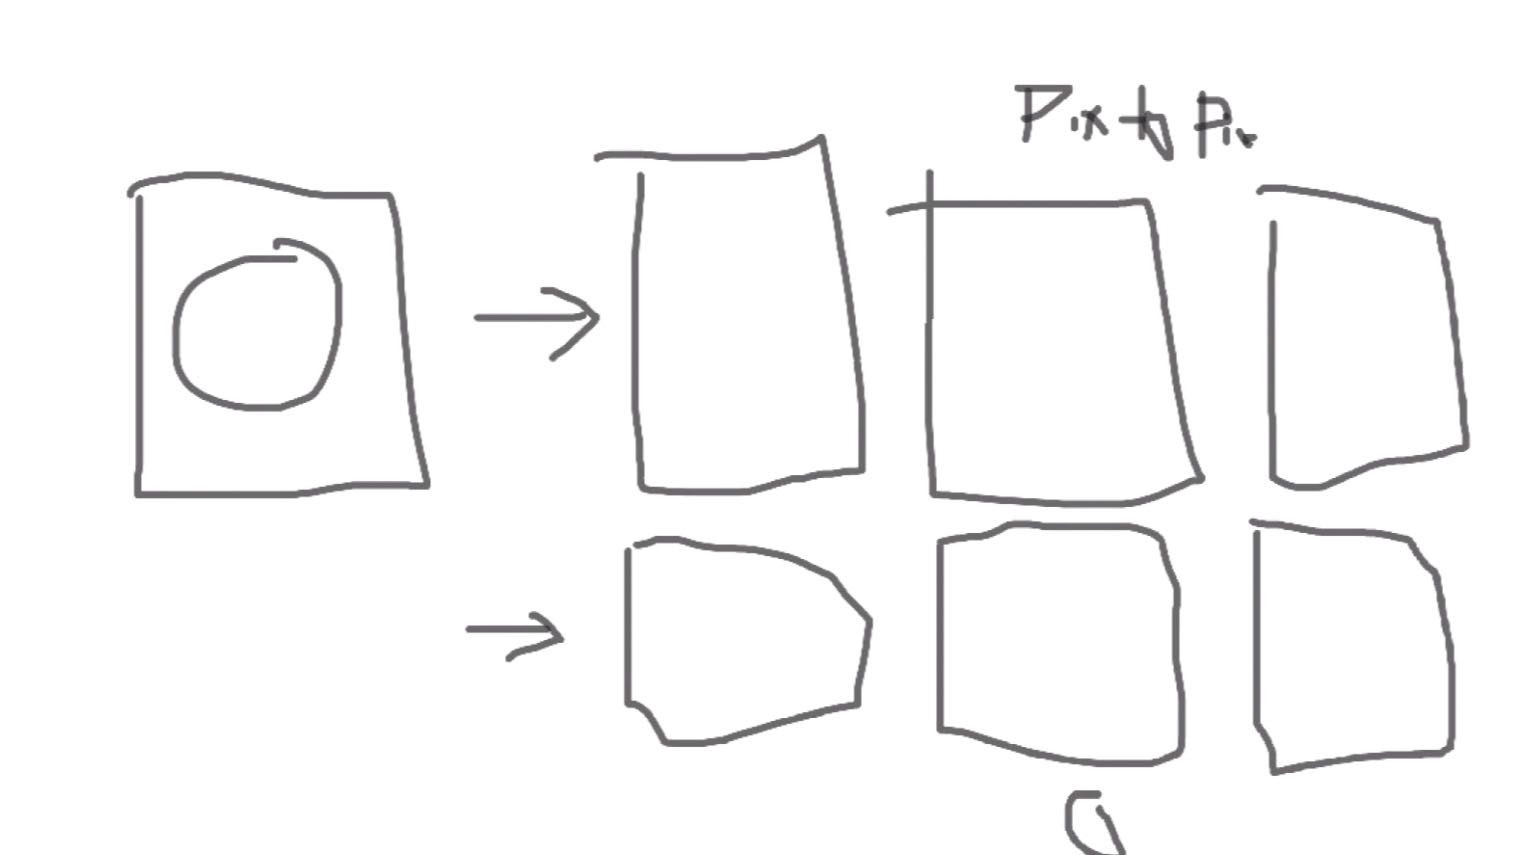
\includegraphics[width=.9\linewidth,height=4.5cm]{images/teaser/sketch.jpg}
    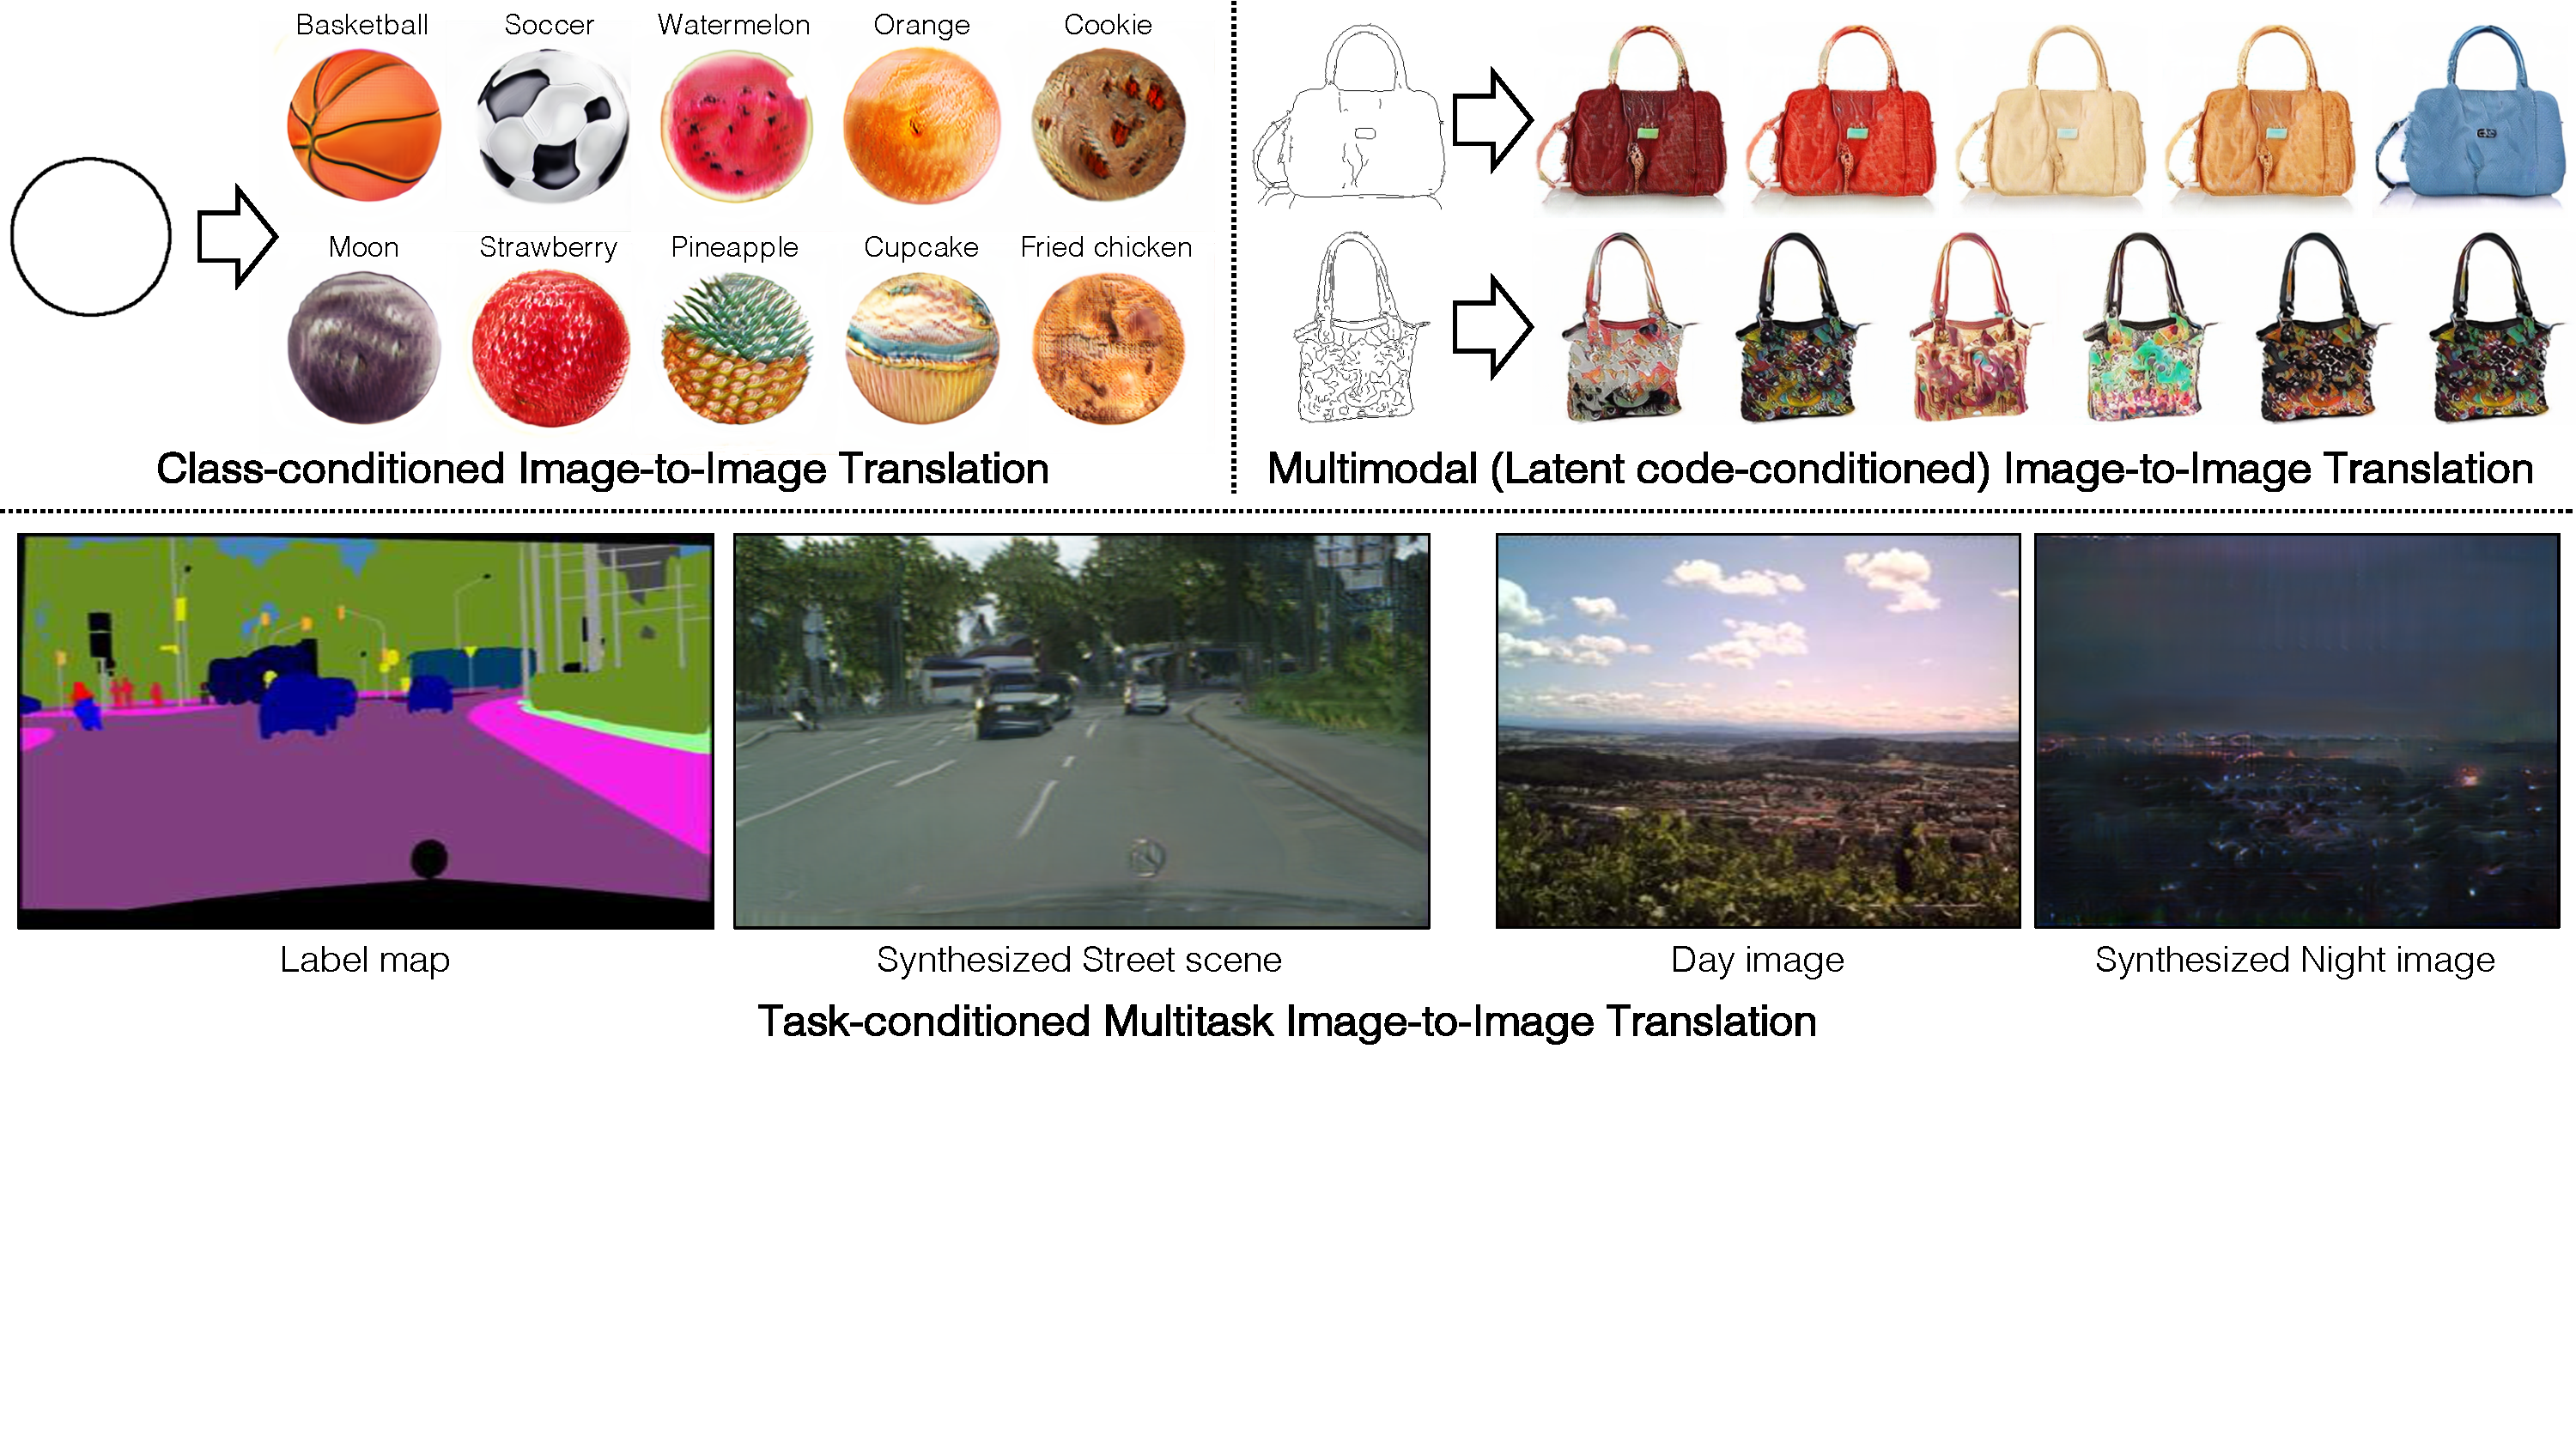
\includegraphics[width=1.\linewidth]{paper_images/fig1.pdf}
    \captionof{figure}{Our proposed GAN-gate method enables conditioning on a variety of conditional image-to-image translation tasks, such as {\bf (top-left)} outline-to-image translation, conditioned on object class {\bf (top-right)} multimodal edge map-to-handbag translation, conditioned on a learned latent code, and {\bf (bottom)} disjoint multitask image-to-image translation. Each of the three examples uses a single generator and discriminator.\label{fig:teaser}}
\end{center}%
}]
    
%%%%%%%%% ABSTRACT
\begin{abstract}
We propose a method that allows us to generate images belonging to multiple domains using a single network. 
Our approach is based on a GAN framework with two separate branches, a fully residual network, and a separate smaller gating network conditioned on the input class that selects residual blocks from the first branch.
The same gating network also conditions the residual blocks of the discriminator network.
We show that such an approach is able to produce high quality multi-class image generation, both in an image-to-image translation task, as well as a random-noise-to-image generation task. 
This method allows for significantly smaller model sizes than previous multi-class approaches by taking advantage of similarities across classes. 
We analyze our gating network to show that it leads to subnetworks based on the residual blocks that are active for a particular class.
%This approach as well as helps inject low dimensional information into a network more effectively than just concatenating channel-wise after replication to match the image dimension. 
Information theoretic results also show it to be a much stronger form of conditioning than naive concatenation. 
We apply our approach on a novel setting of multi-class outline-to-image generation, where baseline solutions fail to generate good results, while our model successfully tackles the multi-class image generation setting. 
\end{abstract}


\begin{figure*}[t]
    \centering
    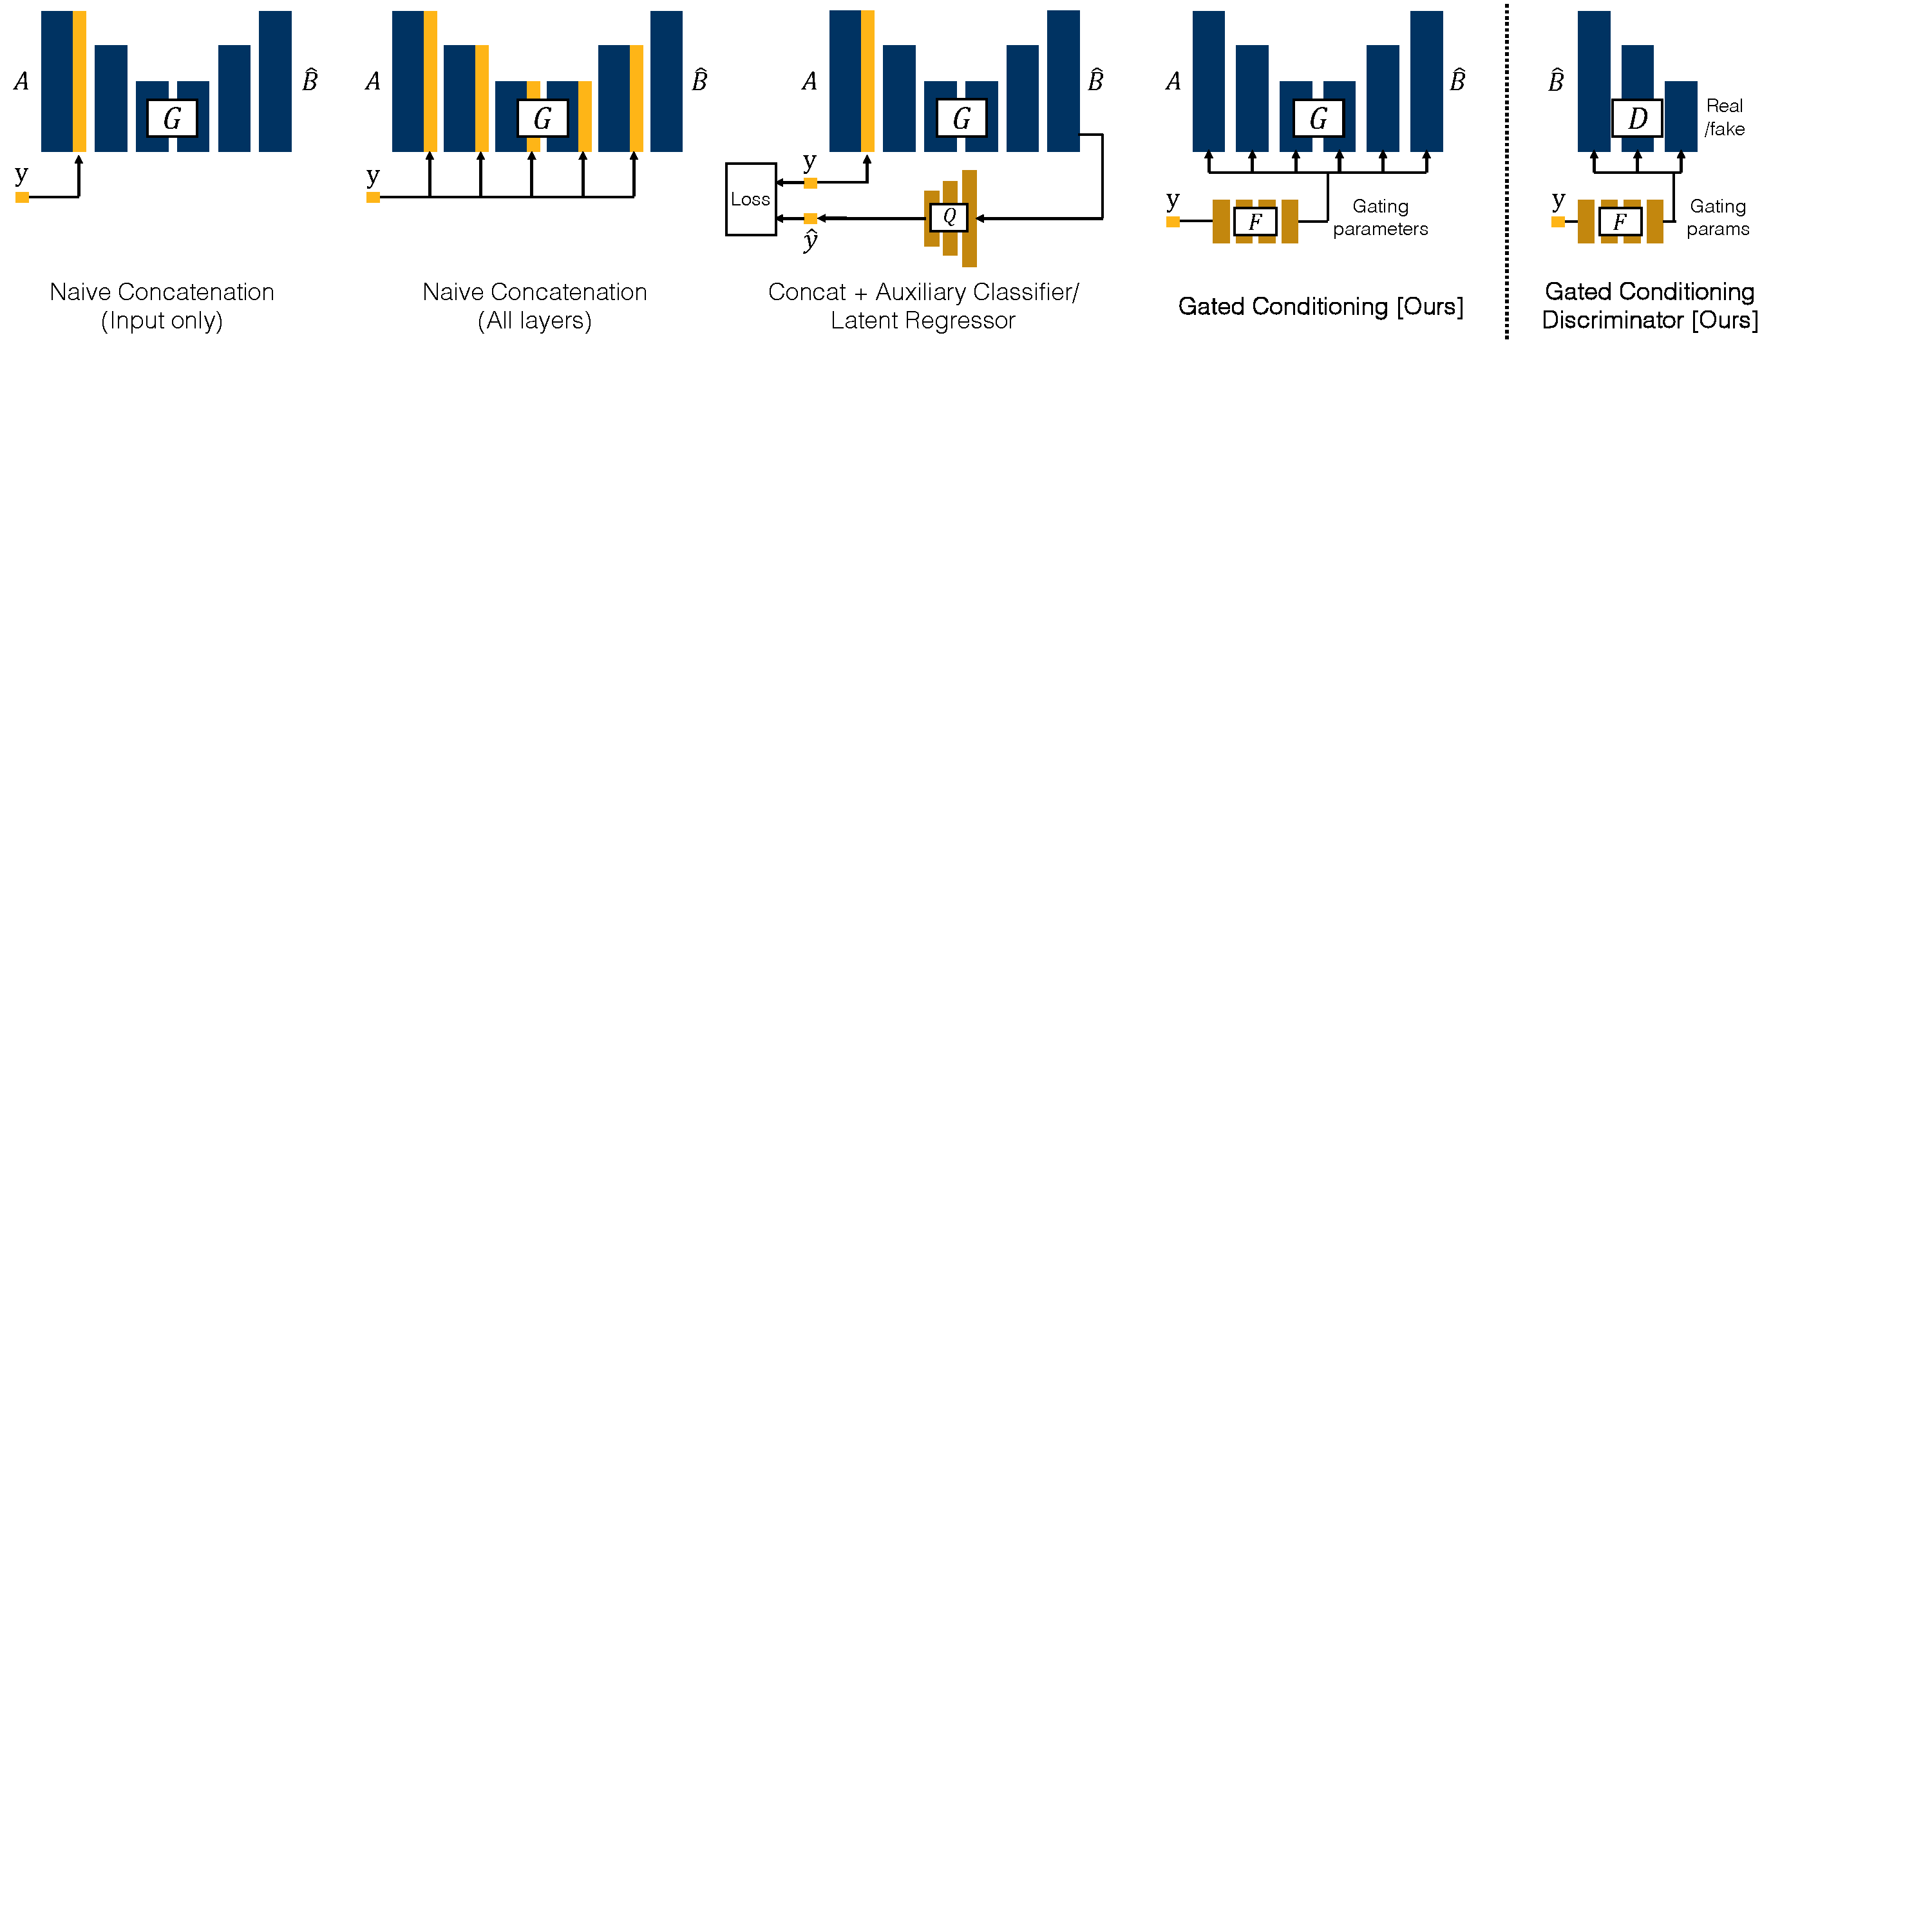
\includegraphics[width=\linewidth]{paper_images/arch_inject.pdf}
    \caption{{\bf Conditioning injection variants.}
    Conditioning information can be incorporated naively in a generator architecture through simple concatenation in {\bf (left)} the input layer only or {\bf (mid-left)} in all layers. {\bf (middle)} The network can be further encouraged to use the conditioning through a learned network, either a classification objective for categorical conditioning~\cite{odena2016conditional,chen2016infogan} or a regression objective for continuous conditioning. {\bf (Mid-right)} We investigate training a network on the conditioning signal, which predicts parameters which are used to guide softly-gated units in the main network. {\bf (Right)} These conditioning options -- concatenation, auxiliary classifier/latent regressor, and our gated conditioning -- can be correspondingly applied to a discriminator.\label{fig:arch-inj} }
    % \vspace{-4mm}
\end{figure*}

\section{Introduction}
Generative methods have made huge strides in the last few years driven by the success of Variational Autoencoders (VAEs)~\cite{kingma2013auto} and Generative Adversarial Networks (GANs)~\cite{goodfellow2014generative}. 
These methods can generate impressive results but one major challenge is that quality degrades quickly when the diversity of training data (e.g., number of object/scene classes) increases. 
It is a common practice in the domain of image conditional generations to train different models for different datasets \cite{goodfellow2014generative,isola2016image2image,karras2017progressive,zhu2017toward,zhu2017unpaired,wang2018video} meaning the number of parameters scales linearly with the number of classes. 
% A study performed in \cite{ghosh2017multi,metz2017unrolledGAN} demonstrated that even in a simple 1D \& 2D Mixture of Gaussians settings, state-of-the-art GAN techniques were not able to generate samples from all the components of the mixture. 
%However their proposed method still involved training multiple generators.
An ideal scenario in such settings would involve a single network which could share parts of the network responsible for operations shared between the various classes, while unsharing the discrete parts of the network which are responsible for class specific operations.

Such a scenario was analyzed in the realm of Image Classification by Veit et al.~\cite{veit2016residual} where they performed incision experiments on a pretrained ResNet architecture \cite{he2016deep}, demonstrating that certain paths in the network played a more important role for certain classes, inferring that ResNets behave like an ensemble of several partially disjoint networks for image classification. 
In this paper we analyze the implications of the observations of \cite{veit2016residual} on a Generative Modeling scenario. 
We analyze GANs on a 1D Mixture of Gaussians dataset as used in \cite{ghosh2017multi}, and discover that the removal of certain blocks of the generator correspond to the disappearance of certain modes in the generated distribution.
We thus introduce a simple {\em soft gating} mechanism where based on the conditioning input (e.g., the class of the object) a hypernetwork predicts which parts of ResNet to use for that particular conditioning.
We explore and analyze different types of gating, including a {\em blockwise} and {\em channelwise} gating, a multiplicative and a scale+bias types of soft weighting as well as other related methods like AdaIn~\cite{huang2017arbitrary,huang2018multimodal}. We show that a channelwise multiplicative gating performs best for our task. We further show that better results are obtained if gating is applied not not only for a ResNet-based generator but also for a ResNet discriminator.


We further introduce a new task of generating multi-class images from rough outline scribbles where gating is particularly useful due to class ambiguities in the mapping. Fig.~\ref{fig:teaser} (top left) shows one such example where the same simple scribble yields different outputs of a generator conditioned on ten different classes.
In the case of the InfoGAN~\cite{chen2016infogan} setting, which was previously shown to produce limited texture variation~\cite{ghosh2017multi} with naive concatenation-based conditioning, our method produces diverse generations, as shown in Fig.~\ref{fig:teaser} (top right).
In addition, we also introduce the {\em multi-task image-to-image translation}. In its original setting \cite{isola2016image2image}, different trained models had to be introduced for the different translation tasks. Our gating mechanism enables good performance on each task by activating appropriate task-specific blocks and channels (Fig.~\ref{fig:teaser} bottom).

%whereby the rough scribbles divulge almost no information about the class.



%%The technique presented a scenario in which we could generate multiple modes for a single dataset but it could further be used for generating multiple modes from a dataset consisting of multiple classes and the hypernetwork could choose the blocks needed for a particular class. 




%%Furthermore we perform a systematic analysis of all meaningful gating mechanisms and other forms of conditioning in the setting of a image conditioned generative model. This paper also finds that gating also enables the discriminator to provide better class conditioned gradients back to the generator for high quality generations.


% Generative methods have made huge strides in the last few years driven by the success of Variational Autoencoders (VAEs)~\cite{kingma2013auto} and Generative Adversarial Networks (GANs)~\cite{goodfellow2014generative}. 
% While these methods can generate impressive results, one major challenge is that quality degrades quickly when the diversity of training data (e.g., number of object/scene classes) increases, especially when the manifold of the multi-class distribution of images drawn from the ground truth distribution is not continuous. \ow{um... I don't really get this previous sentence}

% We propose a solution to generate multi-class images using a form of class conditioning that outperforms prior class conditioned GANs while requiring significantly fewer parameters than using a single GAN per-class. 
% To do this, we take advantage of the fact that different classes will share similar visual features, and propose an architecture wherein a fully-residual GAN generator and discriminator, is combined with a second ``gating'' network, which determines how the network is conditioned on the input class.

% We compare various forms of gating, such as concatenating one-hot class information, auxillary classification, \todo{...}.

% We evaluate our gating approach on a number of applications \todo{...}
% \ow{discuss evaluation and findings}
%



In summary, our contributions are:
\begin{itemize}
\item An in-depth analysis of the role of gating networks in generative modeling.
\item A novel architecture using a gating hypernetwork that can generate diverse multi-class results both when classes are known a-priori, or are derived from the data in an unsupervised fashion (similar to InfoGAN~\cite{chen2016infogan}).
%\item Incision experiments on a trained Residual Generator based GAN on the 1D Mixture of Gaussians to show certain blocks correspond to certain modes in the generated distribution.
%\item Introduction of the Gated Residual Blocks and the Hypernetwork to predict the corresponding alphas on the Generator and Discriminator.
\item Introduction of a new image-to-image translation task of generating realistic images from very rough outline scribbles.
\end{itemize}

\begin{figure*}[t]
    \centering
    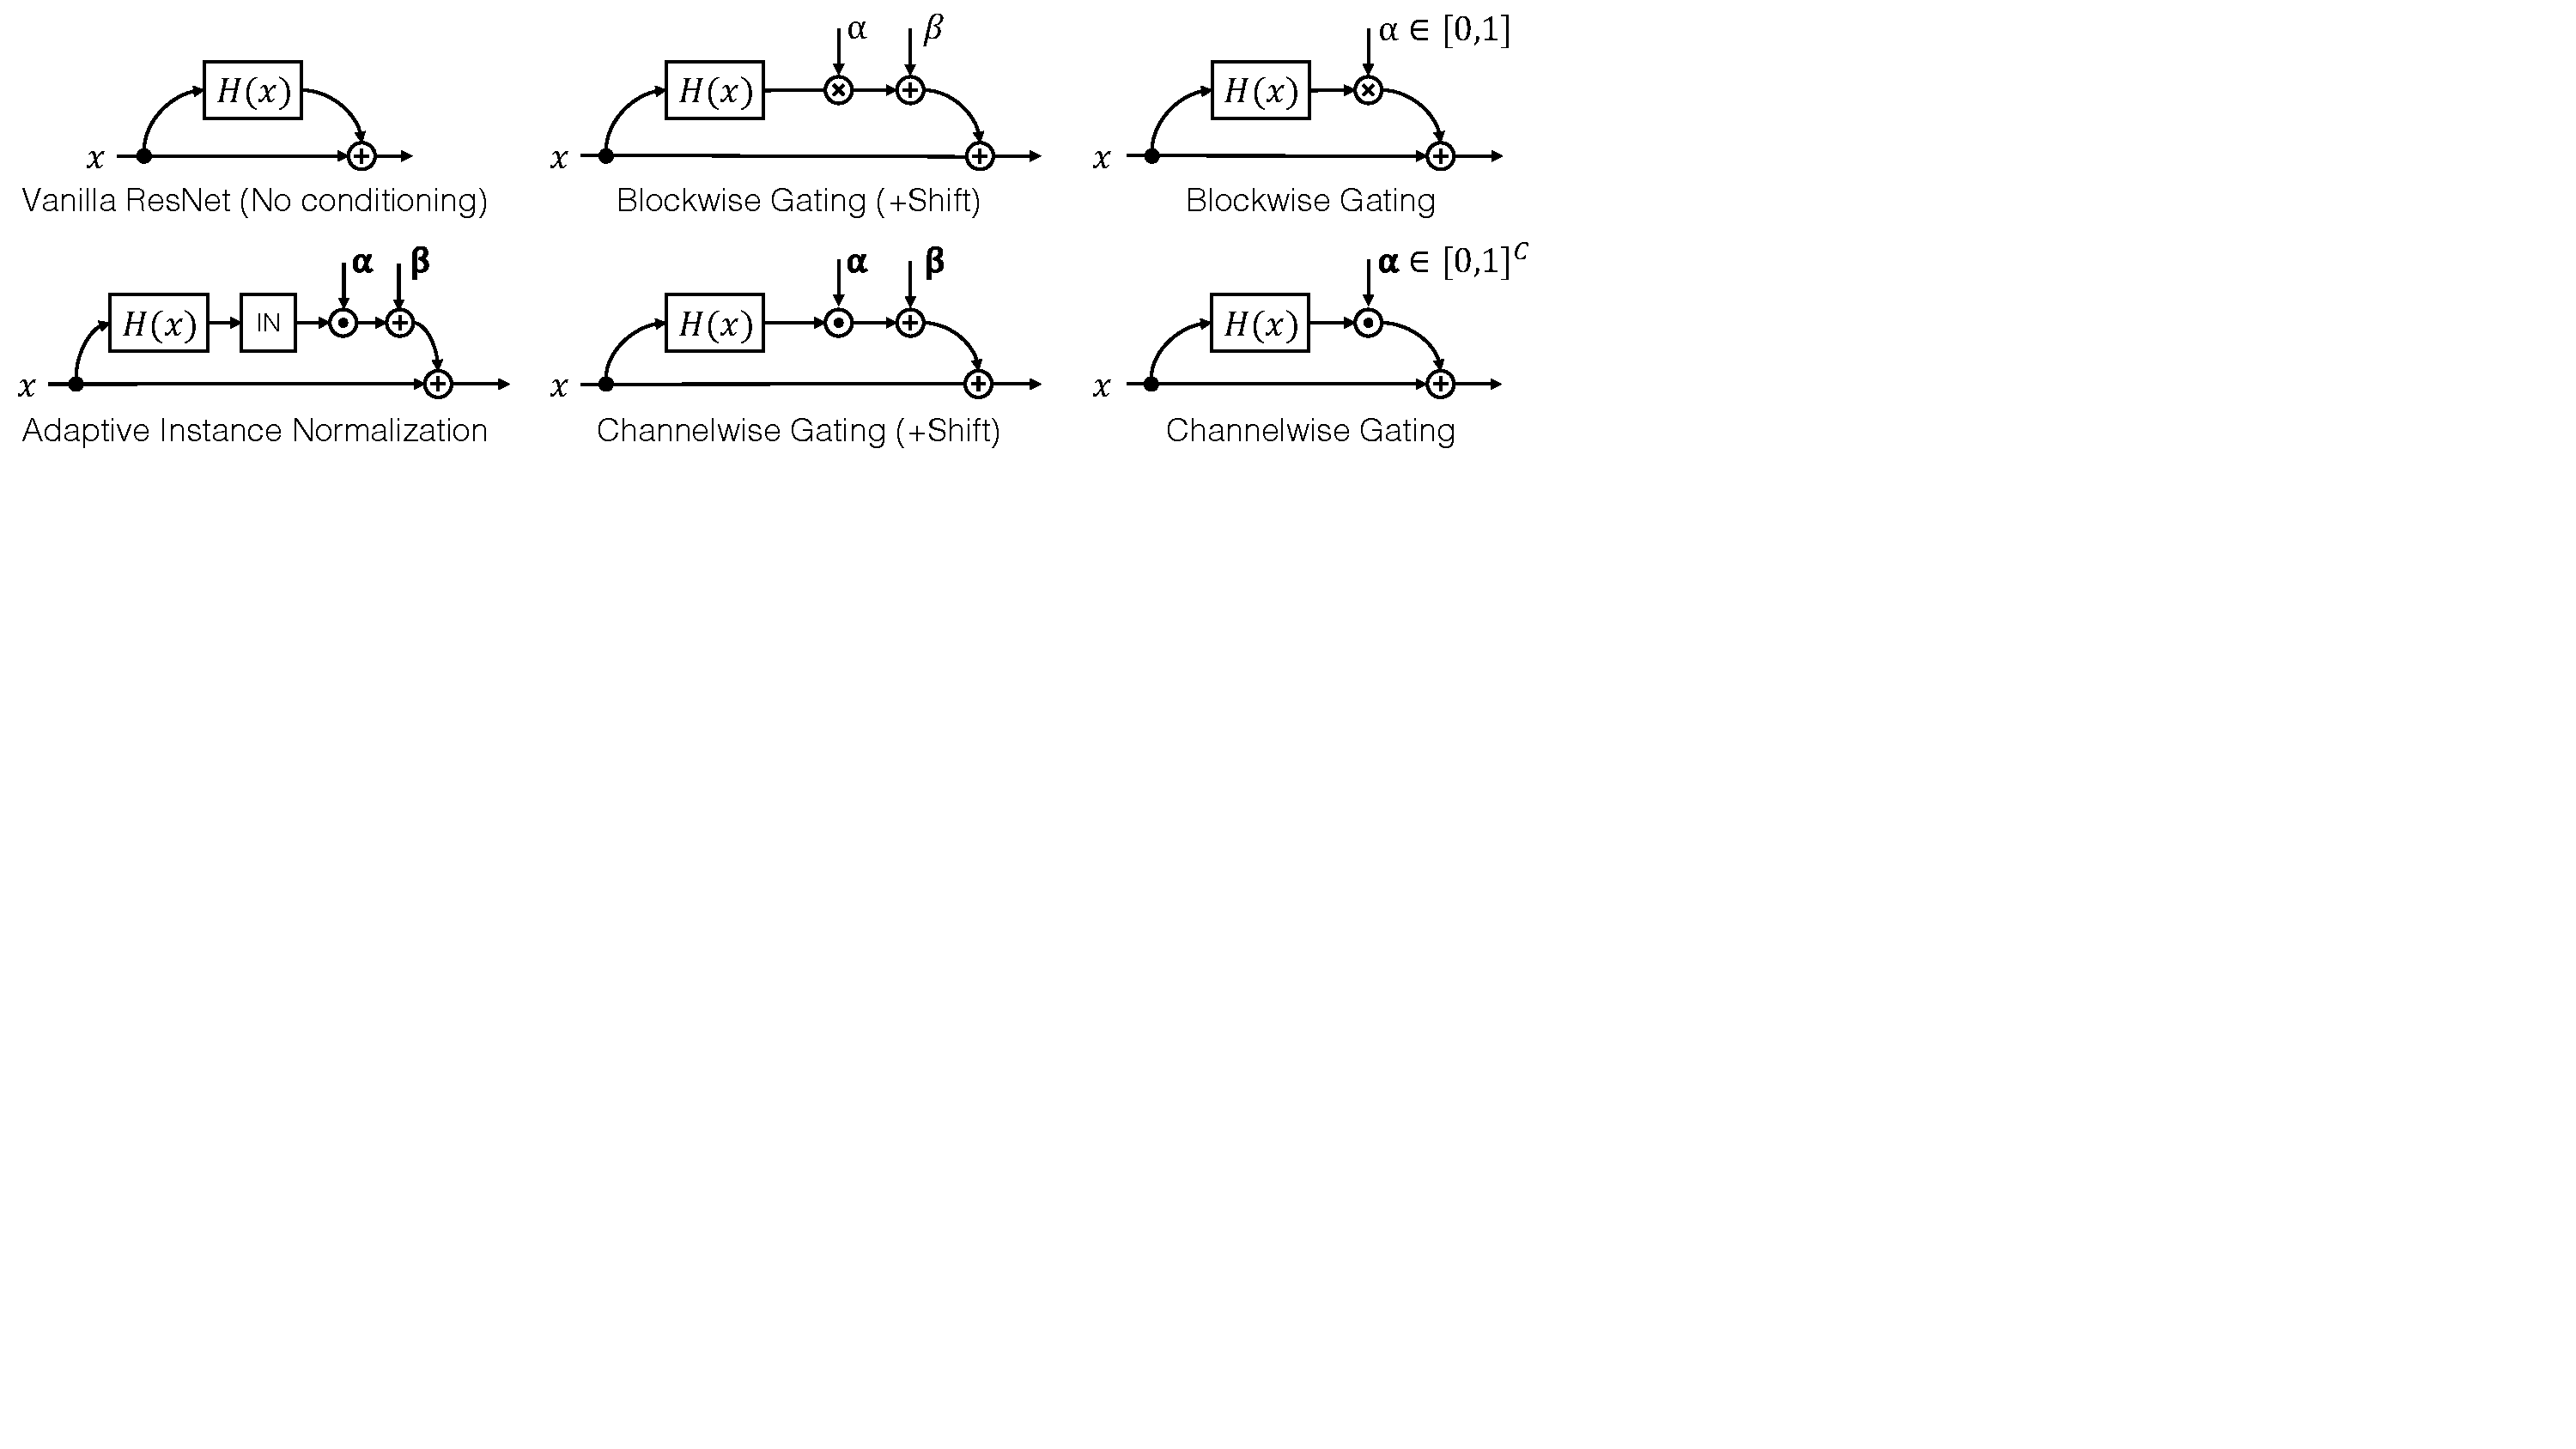
\includegraphics[width=\linewidth]{paper_images/arch_gate.pdf}
    \caption{
    % {\bf Incorporating soft-gating into residual blocks.} \rz{Order got changed, may or may not need to add key for hadamard product}
    {\bf (Top-left)} A ``vanilla" residual block without gated conditioning parameters modifies signal $x$ into $x+\mathcal{H}(x)$. Conditioning with concatenation uses this setup. {\bf (Top-mid)} The $\mathcal{H}(x)$ block is softly-gated by scalar parameter $\alpha$ and shift $\beta$. {\bf (Top-right)} Only the gating is used, without bias. {\bf (Bot-left)} Adaptive Instance Normalization~\cite{huang2017arbitrary} applies a channel-wise scaling and shifting after an instance normalization layer. {\bf (Bot-mid)} Channel-wise gating adds restrictions to the range of $\mbox{\boldmath $\alpha$}$. {\bf (Bot-right)} We find that channel-wise gating (without added bias) to empirically produce the best results.\label{fig:arch-gate} }
    % \vspace{-4mm}
\end{figure*}

\section{Related Work}

\paragraph{Conditioned Image Generation}
Pix2pix \cite{isola2016image2image} introduced a set of tasks whereby the pixels of the input in a different domain corresponded to the pixels of the generated image.
As a result, image-to-image translation methods have exploded in popularity, as many applications can be expressed in this framework.
However, one problem with the original Pix2pix formulation is that the quality degrades quickly with increased class diversity. 
We build upon these ideas by proposing a new architecture and gating scheme that allows for high quality multiclass image generation. 

\paragraph{Mode Collapse} is a major challenge for GANs \cite{goodfellow2014generative}, where the diversity of the generated results is limited and only a portion of the training set is utilized. 
Several techniques deal with this issue, the best performing among those include Spectral Normalization \cite{zhang2018self,miyato2018spectral} which normalizes the spectral norms of the layers to stabilize training, MAD-GAN \cite{ghosh2017multi} which introduces multiple generators, BicycleGAN \cite{zhu2017toward} which reconstructs the latent code from the generation using two cycles, and MUNIT \cite{huang2018multimodal} which introduces a factorized latent space for content and style for producing variations.

An alternative proposal is to add a predictor from the output to the conditioner, to prevent the model from ignoring the condition. This has been explored in the classification setting in Auxiliary-Classifier GAN (ACGAN)~\cite{odena2016conditional} and regression setting with InfoGAN~\cite{chen2016infogan} and BiGAN (``latent regressor" model)~\cite{dumoulin2016adversarially,donahue2016adversarial}, and is one half of the BicycleGAN model~\cite{zhu2017toward}. We explore a complementary approach of architectural modification.

% \ow{not clear to me why it starts with mode collapse... dangerous as we also have it in our results, except the infogan case. I think that this should be changed into an infogan related work section and moved below.}

%but needed far more details such as in the case of edge to handbags generation task it needed texture strokes inside the bag as well to be able to produce high quality diverse generations
%Other forms of conditioning have been introduced in \cite{wang2018video} whereby rough triangles and sparse edges are enough to generate high quality videos. We explore the situation in which the input scribble is extremely sparse and multiple classes can have very similar input scribbles for instance in the case of balls the input scribble is just the outline in the shape of a circle.

%Our architecture also differs from previous art in the form of the architecture whereby all the blocks are residual including the downsampling and upsampling. Previous literature mostly used the residual blocks in the bottleneck layer of an Encoder Decoder structure. The number of channels in the networks doesn't change with the change of resolution as in the original Resnet architecture \cite{he2016deep} in order to ease the learning of the gating mechanism. 

\paragraph{Gating Mechanisms}
%Residual Networks \cite{he2016deep} introduced a new set of architectures that enabled training of very deep networks.
Prior work has demonstrated that in ResNets, some paths are more important for particular classes~\cite{veit2016residual}, and has used this to develop a hard gating mechanism~\cite{veit2018adaptive}.
We provide a further analysis of gating mechanisms, in the context of GAN image generation, as opposed to image classification.

Our approach is also related to Adaptive Instance Normalization (AdaIn) ~\cite{huang2017arbitrary}, which has been used to great success in style transfer~\cite{huang2017arbitrary} and multimodal image-to-image translation~\cite{huang2018multimodal}.
However, we use a fully residual architecture, and employ soft gating both in the generator and discriminator. 
%Although previous work has explored the idea of gating via AdaIN in the generator but our techniques also involves using gating in the discriminator as well. 
We evaluate AdaIn style gating among other possible choices with our fully residual architecture, and show that channel gating achieves superior performance for our task.

Another gating mechanism, FiLM~\cite{perez2017film}, was introduced in the context of Visual Question Answering.
In this case, the gating mechanism is conditioned on the input question.
Gating also plays an important role in natural language processing: LSTMs \cite{hochreiter1997long} and GRU \cite{cho2014learning}.


% The seminal work by \cite{miyato2018spectral}, introduced spectral normalization which normalizes the weights of the network such that the maximum eigen value of the resulting set of weights is bounded. It helped enormously in stabilizing the training of GANs and albeit they only applied spectral normalization to the discriminator, SA-GAN \cite{zhang2018self} applied it to both the generator and discriminator and showed superior generative modeling performance over several tasks. SA-GAN further introduced the self attention layer based on the innovative transformer network and showed not only better geometric properties being modeled by the GAN but also allowing Multi-Class generations.
% The Projection Discriminator \cite{miyato2018cgans} based Conditional GANs altered the naive model of concatenating the condition provided to the discriminator via a generalized bilinear projection between the condition and the features extracted from the image thereby providing more finegrained gradients suitable for training the generator to produce class conditional and better resolution images. 
% MAD-GAN \cite{ghosh2017multi} introduced multiple generators and showed an innovative experiment whereby they mixed images from 3 classes and the 3 generators could disentangle the classes and each of the generators generated much sharper images from a particular class than a single generator with similar capacity could. 

% %moved from intro
% To combat this challenge a solution called MAD-GAN \cite{ghosh2017multi} was proposed which dealt with the issue via multiple generators whereby the discriminator distributed the modes and classes in the data distribution among the various generators. 
% Although MAD-GAN was a novel solution to deal with discontinuities in the manifold of the multi-class data distribution, the solution came with its flaws, supreme among them was the reduced scalability in the case the structure was not shared among the different classes, the generators couldn't share the initial layers' parameters and therefore was limited by GPU capacity and in practice going more than 5-6 generators was difficult. 

% In another line of papers which helped build the ideas in this paper are the research on Residual Networks \cite{he2016deep} which introduced a set of architectures which allowed extremely deep networks to be trained upto hundreds of layers which was earlier assumed to be extremely difficult because of the problem of vanishing gradients in deep networks. The residual connection allowed a unadulterated gradient backpropagation pathway which enabled training of ultra deep networks. A thorough analysis of residual networks by \cite{liao2016bridging} showed that residual networks have similar connections to unrolled recurrent neural networks without weight sharing and is very similar to how computation unfolds in human brains. Veit et al. \cite{veit2016residual} did a set of innovative incision experiments whereby they removed some blocks and allowed only the skip connection to be active in a trained Residual Network and they were able to demonstrate that even after removing some layers there a very miniscule reduction in the classification accuracy while a similar incision in a VGG network \cite{simonyan2014very} which doesn't have skip connections led to almost random outputs in the task of classification. \cite{veit2016residual} also demonstrated that residual networks behave as an ensemble of several shallower networks. \cite{veit2018adaptive} used the concepts introduced in \cite{veit2016residual} to introduce a discrete gating mechanism in deep residual networks based on the Gumbel-Softmax approximation to make the discrete decision differentiable. Their approach allowed redundant computations in the residual blocks to be reduced and to use only few of the blocks in the trained network during testing phase of the neural network. \cite{de2017modulating} introduced a technique for modulating the activations of a residual block by predicting the parameters of batch normalization which they term as Conditional Batch Normalization. In a similar vein \cite{perez2017film} also used a similar technique for modulating the activations of the various blocks conditioned on the question in a Visual Question Answering scenario.

% Gating mechanisms have generally been useful for language modeling tasks such as LSTMs \cite{Hochreiter1997LSTM} and \cite{chung2014empirical} which improved language modeling performance over vanilla RNNs. Gating also helped in the case of image recognition as demonstrated in Highway Networks \cite{srivastava2015highway} albeit it has a lot of resemblance to residual networks. 

% Image manipulation and Generation has seen huge strides in recent years with the advent of Generative Adversarial Networks \cite{goodfellow2014generative}, style transfer networks \cite{gatys2015neural} and image colorization \cite{zhang2016colorful}. iGAN \cite{zhu2016generative} was one of the first very innovative papers that introduced us to a novel technique for editing images using neural networks and preventing the edited images to fall off the natural image manifold. Pix2pix \cite{isola2016image2image} introduced a novel network based on GANs which could translate images on a plethora of datasets such as edges to handbags, semantic layout to photo realistic images and day to night. Cutting edge techniques on similar lines include \cite{wang2018video} which can translate from Video to Video such as from pose sequences to a person dancing or from semantic layouts to photorealistic road scenes. InfoGAN \cite{chen2016infogan} introduced a novel network based on GANs and Information Theoretic principles which could disentangle modes in the data distribution based on an unsupervised objective but showed poor performance in being able to disentangle modes and produce stochastic variations in the setting of pix2pix which is known to collapse to a single output for a particular input whereas ideally it should be a distribution. Bicycle GAN \cite{zhu2017toward} introduced 2 cycles which was able to produce stochastic generated outputs in the case of image to image translation. Another innovation was CycleGAN \cite{zhu2017unpaired} which allowed unpaired image to image translation as well as unpaired domain transfer which enabled several transformations which wasn't possible earlier. 



% \section{Preliminaries}
\newcommand{\addSubFigHalf}[3]{\begin{subfigure}[t]{.45\linewidth}
   \includegraphics[width=\linewidth]{#1}
   \caption{#2}\label{#3}\end{subfigure}
}


One aspect of residual networks is that information can bypass layers, forming essentially an ``ensemble'' of several shallower networks.
Veit et al.~\cite{veit2016residual} showed in a classification setting, that classification performance is largely maintained even when fully removing some residual blocks.
We investigate whether this aspect can lead to more efficient parameter usage for multi-class image generation, by using fully residual networks for both generator and discriminators in a GAN network.
Instead of fully removing residual blocks, we evaluate a number of soft-gating mechanisms.
%with a whereby a hypernetwork gets the condition modulates the feature activations of the residual blocks i.e. the output of the standard residual block was modified from $x+f(x)$ to  $x+\alpha . f(x)$ where the set of alphas for each of the residual block is predicted by the hypernetwork. 


\paragraph{Relationship to conditioning}
This approach can be seen as form of conditioning. 
Conditioning by concatenation is a weak form of conditioning because by information theoretic principles, the deeper the network the lesser mutual information is preserved between the conditioning input and the output of the network. To mitigate this issue some other solutions such as the projection discriminator \cite{miyato2018cgans} have been proposed and our residual gate selection block on the discriminator is along similar lines. 


\begin{align}\label{eq:ganObjective}
     \min_{\theta_g}\max_{\theta_d}\; & V(\theta_d, \theta_g) := \E_{x \sim p_{d}} \log D(x; \theta_d) \nonumber \\&
     + \E_{z \sim p_z } \log \big( 1 - D(G(z; \theta_g) ; \theta_d)\big) 
\end{align}
\paragraph{GANs:} 
Here we present a brief review of GANs~\cite{goodfellow2014generative}. Given a set of samples $\mathcal{D} = (x_i)_{i=1}^n$ from the true data distribution $p_d$, the GAN learning problem is to obtain the optimal parameters $\theta_g$ of a generator $G(z;\theta_g)$ that can sample from an approximate data distribution $p_g$, where $z \sim p_z$ is the prior input noise (\eg samples from a normal distribution). In order to learn the optimal $\theta_g$, the GAN objective (Eq. \eqref{eq:ganObjective}) employs a discriminator $D(x; \theta_d)$ that learns to differentiate between a {\em real} (from $p_d$) and a {\em fake} (from $p_g$) sample $x$. The overall GAN objective is:


The above objective is optimized in a block-wise manner where $\theta_d$ and $\theta_g$ are optimized one at a time while fixing the other. For a given sample $x$ (either from $p_d$ or $p_g$) and the parameter $\theta_d$, the function $D(x; \theta_d) \in [0, 1]$ produces a score that represents the probability of $x$ belonging to the true data distribution $p_d$ (or probability of it being real). The objective of the discriminator is to learn parameters $\theta_d$ that maximizes this score for the true samples (from $p_d$) while minimizing it for the fake ones $\tilde{x} = D(z; \theta_g)$ (from $p_g$). In the case of generator, the objective is to minimize $\E_{z \sim p_z}\log \big( 1 - D(G(z; \theta_g) ; \theta_d) \big)$, equivalently maximize $\E_{z \sim p_z} \log D(G(z; \theta_g) ; \theta_d)$. Thus, the generator learns to maximize the scores for the fake samples (from $p_g$), which is exactly the opposite to what discriminator is trying to achieve. In this manner, the generator and the discriminator are involved in a minimax game where the task of the generator is to maximize the mistakes of the discriminator. Theoretically, at equilibrium, the generator learns to generate real samples, which means $p_g = p_d$.

\subsection*{Residual Networks:}
There was the standard degradation problem in deep neural networks that even after adding more layers to a network the performance of the network doesn't increase . Residual Networks\cite{he2016deep} address the degradation problem by introducing a deep residual learning framework. Instead of hoping each few stacked layers directly fit a desired underlying mapping, they explicitly let these layers fit a residual mapping. Formally, denoting the desired underlying mapping as H(x), they let the stacked nonlinear layers fit another mapping of $F(x):=H(x)-x$. The original mapping is recast into $F(x)+x$. The hypothesis is that it is easier to optimize the residual mapping than to optimize the original mapping. To the extreme, if an identity mapping were optimal, it would be easier to push the residual to zero than to fit an identity mapping by a stack of nonlinear layers.


We show an interesting set of experiments in the 1D setting of Mixture of Gaussians as was performed in \cite{ghosh2017multi}. A model was trained with the generator composed of residual blocks and then in line with the experiments performed in \cite{veit2016residual} we removed certain residual blocks and allowed the information to flow through the skip connection and we found that removal of certain modes corresponded to the removal of certain residual blocks hence supporting the arguments in \cite{veit2016residual} that residual networks behave as an ensemble of several shallower networks even in the case of generative models.


\begin{figure}[t]
    \centering
    \addSubFigHalf{Picture33.png}{Generated Samples from the trained Generator}{fig:1d_gen} 
    \addSubFigHalf{Picture3.png}{Generated Samples from the trained Generator with one of the blocks removed}{fig:1d_gen_rem} 
    \caption{Generations in MoG 1D setting}
    \label{fig:onedexperiment}
    \vspace{-3mm}
\end{figure}
\paragraph{1D experiment:}
We first evaluate the effect of a gating network in a simple scenario where the data distribution is a 1D mixture of Gaussians. 
We train \model{} in this simple setting, analyze the effect of removing different blocks via the gating network, in the vein of \cite{veit2016residual}.
We observe in Figure ~\ref{fig:onedexperiment}, when some residual blocks were disabled (and only the skip connection of that block was activated), it led to the disappearance of particular modes from the data distribution. 
Removal of groups of blocks led to the disappearance of clusters of modes from the generated distribution. 

% \begin{figure*}%[ht!]
%     \centering
%     \addSubFigHalf{Picture13.png}{Gated Residual Blocks for the Generator}{fig:gru_gen} 
%     \addSubFigHalf{Picture14.png}{Gated Residual Blocks for the Discriminator}{fig:gru_dis} 
%     \caption{Gated Residual Blocks in Generator and Discriminator}
%     \label{fig:model}
%     \vspace{-3mm}
% \end{figure*}


\paragraph{MNIST experiment:}
Our experiments with the gate selection block on the quintessential MNIST dataset show its efficacy in a limited setting, we further show that infogan based network could be applied to the pix2pix experiments which was earlier known to produce the delta distribution and only a single plausible output \cite{ghosh2017multi}. The resulting infogan based network was able to produce stochastic variations on the generated samples for the task of edges to handbags. We further show the efficacy of the model in the case when we have explicit class information and use it for a novel task of multi-class scribble to image generation. 






\begin{figure*}[t]
    \centering
    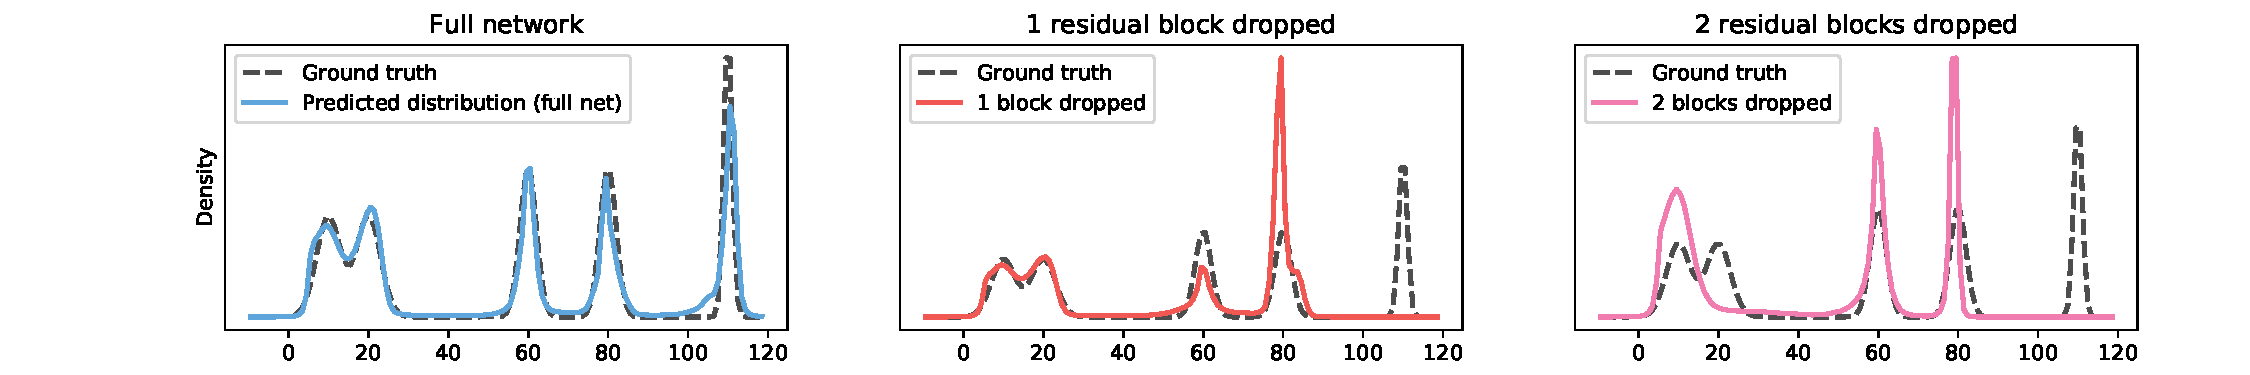
\includegraphics[width=\linewidth,trim={2.2cm 0 1.8cm 0},clip]{paper_images/mog.pdf}
    % 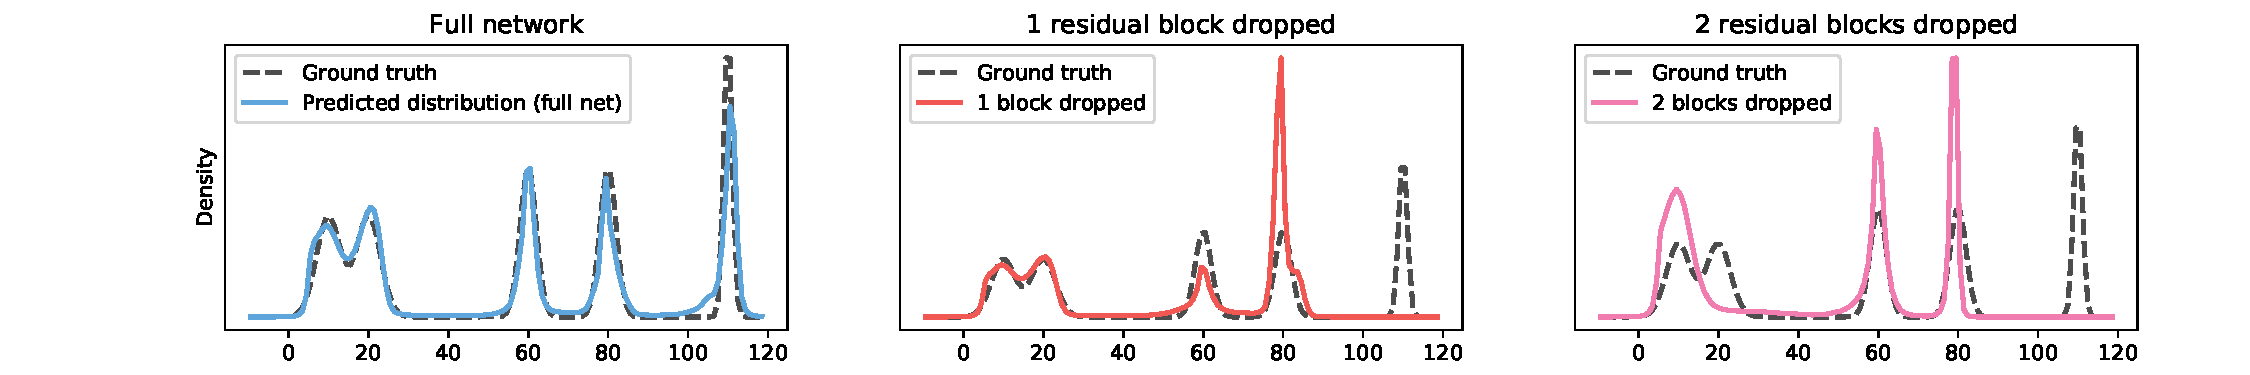
\includegraphics[width=\linewidth]{paper_images/mog.pdf}
    \caption{{\bf 1D Mixture of Gaussians experiment} {\bf (Left)} Samples from a residual network (blue-dotted) closely approximate the training distribution (black). {\bf (Middle)} Removing one residual block removes one mode of the predicted distribution. {\bf (Right)} Removing two blocks results in drop of two modes. Note that the samples stay ``on-manifold" of the ground truth distribution.
    }\label{fig:onedexperiment}
    % \vspace{-4mm}
\end{figure*}

\section{Gated Generative Adversarial Network}
\label{sec:methods}
We consider image-to-image translation problems, mapping input image $A$ to output $B \in \mathds{R}^{h\times w\times 3}$, with the benefit of a conditioning vector ${\bf y} \in \mathds{R}^{d}$. We learn this mapping with multi-layer generator $\widehat{B}=\mathcal{G}(A,{\bf y})$. We refer to the feature map at each channel as $X_l\in \mathds{R}^{h_l\times w_l\times c_l}$, where $h_l \times w_l$ is the spatial size of the feature map, and $c_l$ is the number of channels in the layer. 
% The total channels in the network is $C = \sum_l C_l$. 
The conditioning vector ${\bf y}$ can be categorical, expressed as a 1-hot vector, or a continuous vector. 
% , ground truth output $B \in \mathds{R}^{H\times W\times 3}$, generator $\mathcal{G}$, output $\widehat{B}=\mathcal{G}(A,y)$.

% \subsection{Conditioning injection variants}

The structure of the generator plays a critical role in the effectiveness of the conditioning. We systematically explore several variants, as illustrated in Figure~\ref{fig:arch-inj}. 



\subsection{Naive concatenation}
There are many ways that the conditioning vector $\bf y$ can be integrated into the network. 
The most straightforward is to spatially replicate the vector into a tensor of appropriate size, and concatenate it to the input layer~\cite{zhu2017toward,choi2017stargan}.

A potential weakness of concatenating at the {\em input only} is the large distance between the conditioner and the output, which can lead to the generator ignoring the conditioner during learning. A possible solution is to simply concatenate the conditioner into every layer. This has been previously explored in ~\cite{zhu2017toward}.

\subsection{Recovering the conditioning vector}

% \paragraph{Auxiliary classifier or latent regressor for conditioning vector recovery}
An alternative is to encourage the use of the conditioner through the objective function. 
For example, this can be done by the addition of a hypernetwork, $Q$, charged with recovering the conditioner from the output $\widehat{B}$. 
A loss $\ell$ is added to the optimization between ground truth $y$ and predicted $\hat{y}$.
This term encourages the output to contain enough information about the conditioner. This approach has been explored in the classification setting with Auxiliary-Classifier GAN (ACGAN)~\cite{odena2016conditional}, regression setting with InfoGAN~\cite{chen2016infogan} and BiGAN (``latent regressor" model)~\cite{dumoulin2016adversarially,donahue2016adversarial}, and is one half of the BicycleGAN model~\cite{zhu2017toward}. Here we explore an alternative and more general approach, based on gating.

\ow{what is the problem with the above approach that leads us to propose the next}
\eli{I added a sentence but maybe we can say something stronger? Did we ever try ACGAN on the multi-class task? If yes and it didn't work, maybe mention here?}

\subsection{Conditioning with Soft-Gating (Proposed)}
%The methods above do not fundamentally modify the structure of the network. 
In ResNets, an input feature tensor $X_l$ is modified by function $X_{l+1} = X_l+\mathcal{H}_l(X_l)$.
Changes in resolution are obtained by upsampling or downsampling before the residual block.
We investigate multiple variants of the \textit{learned} gating network, illustrated in Figure~\ref{fig:arch-gate}.
For visual clarity, we omit the layer subscript $l$ in feature tensor $X_l$, residual subnetwork $\mathcal{H}_l$, and the gating parameters $\alpha_l, \beta_l$.

We begin by predicting a scalar $\alpha$ using a learned network $\mathcal{F}({\bf y})$ for each layer of the network:


% We now begin to describe our model which we call Gated Generative Adversarial Networks (GAN-Gate). It is primarily based on an interesting experiment whereby \cite{veit2016residual} showed that the residual networks behave as an ensemble of several shallower networks, and removing a few residual blocks at test time performed highly competitive to the original network itself. This implies that, perhaps, given a GAN architecture with residual blocks as its components, it is possible to {\em automatically} learn a mixture of shallower networks {\em conditioned} on the modes of the data distribution or the tasks we are interested in. This is exactly the objective that GAN-Gate achieves. More precisely, it automatically learns a mixture of shallower networks where each mixture component (a shallow network) is focused on generating data either from a mode or a task; depending on whether we are interested in {\em intraclass} or {\em interclass} variations. To this end, we first propose an architecture for GANs entirely based on residual blocks which is capable of generating highly competitive samples form image-to-image translation task compared to other baselines. Then, we propose to use a simple yet powerful {\em gating mechanism} over a subset of residual blocks where the gating automatically decides which blocks to {\em focus on} for a given condition. Note, this gating is learned automatically from the data. In the end, we also show that the gating mechanism provides an effective way to maximize mutual information in the {\em InfoGAN} objective, which otherwise was not possible.


\begin{equation}
X + \alpha \; \mathcal{H}(X), \text{where } \alpha \in [0,1]
\end{equation}

If the conditioning vector ${\bf y}$ does not have use for a particular block, it can predict $\alpha$ close to zero, and effectively switch off the layer, and use that layer instead for other classes.
Intuitively, during training, blocks within the main network can transform the image in various ways, and network $\mathcal{F}$ can modulate such that the ``right" blocks are selected.

We can apply the operation channel-wise as well, using a predicted vector {\boldmath$\alpha$}.
This provides additional degrees of freedom for network $\mathcal{F}$, to choose to switch specific changes to channels ``on" or ``off". This is denoted as follows:

\begin{align}
X + \mbox{\boldmath $\alpha$} \odot \mathcal{H}(X), 
\end{align}

where $\odot$ is channel-wise multiplication. We make the corresponding changes in the discriminator as well. 
%Soft-gating has been explored by Veit et al.~\cite{veit2018adaptive} in a classification setting. 
Intuitively, in GANs, this can enable the discriminator to select blocks which effectively judge whether generations are real or fake, conditioned on the class input.
% Via accurate gradients backpropagated to the generator it also enables the generator to generate class conditioned high resolution image samples.
Some blocks can be shared across regions in the conditioning vector, whereas other blocks can specialize for a given class.

We empirically find that channel-wise gating provides the strongest results. 
For completeness, we additionally explore incorporating shifting after the soft-gating, either block-wise using a scalar $\beta$ per layer, or channel-wise using a vector {\boldmath $\beta$} per layer.


%\rz{sentence summarizing why or how}

% \begin{equation}
% \text{AdaIn}(x, \alpha, \beta) = \alpha \big(\frac{x-\mu(x)}{\sigma(x)}\big)+\beta
% \label{eqn:adain}
% \end{equation}

AdaIn layers perform a similar gating task:

\begin{equation}
X + \mbox{\boldmath $\alpha$} \odot \text{IN} (\mathcal{H}(X)) + \mbox{\boldmath $\beta$}, 
\end{equation}

In this case, we constrained each element of {\boldmath $\alpha$} and {\boldmath $\beta$} between $[-1, 1]$\footnote{constraining between \( [0, 1] \) did not provide the best empirical results.}, and an Instance Normalization~\cite{ulyanovinstance} (IN) is applied.
%\rz{Some note about how that didn't work so we did [-1,+1], although I'm not sure how this will fly since it didn't need to be constrained in MUNIT, and our stuff then becomes channel-wise so I'm not sure how to play all this}.


% \begin{figure*}[t]
%     \centering
%     \addSubFigThird{Picture2}{Ground Truth Distribution }{fig:1d_ground} 
%     \addSubFigThird{Picture33.png}{Generated Samples from the trained Generator}{fig:1d_gen} 
%     \addSubFigThird{Picture3.png}{Generated Samples from the trained Generator with one of the blocks removed}{fig:1d_gen_rem} 
%     \caption{{\bf 1D Mixture of Gaussians experiment}}
%     \label{fig:onedexperiment}
%     \vspace{-3mm}
% \end{figure*}


\begin{figure*}[t]
  \centering
  \begin{minipage}[b]{0.5\linewidth}  
  \scalebox{0.84} {
  \begin{tabular}{l c c c c}
  \toprule
    \multirow{3}{*}{\textbf{Method}} & \multicolumn{2}{c}{ {\bf SkinnyResNet}} & \multicolumn{2}{c}{ {\bf EncDec}} \\ \cmidrule(l){2-3} \cmidrule(l){4-5}
% 	& \textbf{Accuracy} & \textbf{Realism} & \textbf{Accuracy} & \textbf{Realism} \\
	& Class. & AMT Fool. & Class. & AMT Fool. \\
	& Acc [\%] & Rate [\%] & Acc [\%] & Rate [\%] \\ \midrule
% 	\cmidrule(l){1-1} \cmidrule(l){2-3} \cmidrule(l){4-5}
    Ground truth & 100.0 & 50.0 & 100.0 & 50.0 \\ \midrule
    1 gen/class & \textbf{\textit{97.0}} & 17.7$\pm$1.46 & -- & -- \\ \midrule
    Concat (In)	& 62.6 & 15.0$\pm$1.4 & 39.2 & 7.5$\pm$1.06 \\ 
    Concat (All) & 64.5 & 15.3$\pm$1.41 & 51.4 & 5.4$\pm$0.88 \\ \midrule
    Cat(In)+Aux-Class & 65.6 & 14.5$\pm$1.5 & -- & -- \\ 
    Cat(All)+Aux-Class & 67.0 & 19.7$\pm$1.42 & -- & --\\ \midrule
    BlockGate(+bias) & 89.6 & 19.6$\pm$1.34 & -- & --\\ 
    BlockGate & {\bf 99.6} & 17.3$\pm$1.61 & -- & --\\ 
    AdaIn & 94.5 & 14.9$\pm$1.47 & -- & --\\ 
    ChanGate(+bias) & 94.1 & 14.8$\pm$1.43 & -- & --\\ 
    ChanGate & \textbf{\textit{97.0}} & {\bf 23.4$\pm$1.99} & 92.7 & 14.1$\pm$1.48 \\ 
	\hline
	\end{tabular} } \\
  \end{minipage}
  \begin{minipage}[b]{0.48\linewidth}
  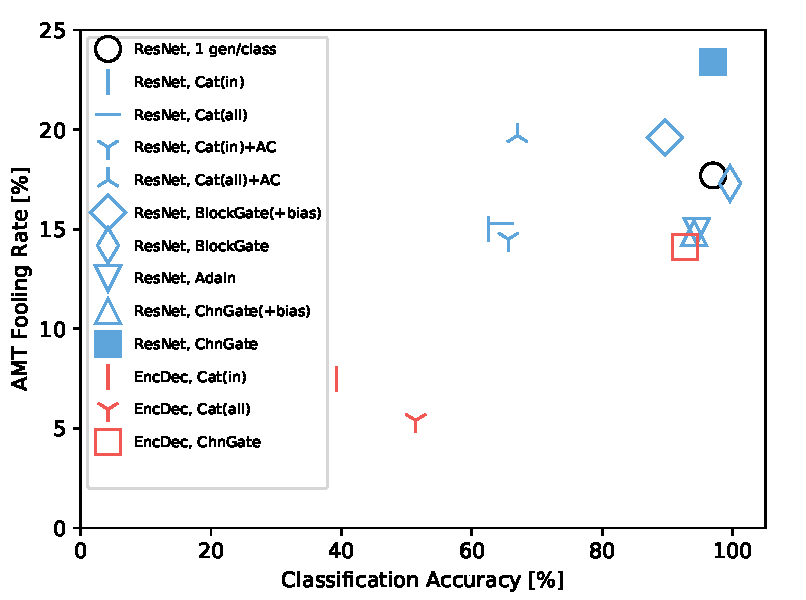
\includegraphics[width=\linewidth]{paper_images/gen_real_vs_acc.pdf} 
  \end{minipage}
%   \vspace{-2mm}
  \caption{\small {\bf Accuracy vs Realism on Outline$\rightarrow$Image task.} We measure generation accuracy by using a pretrained network to check whether the generated image is of the correct class and realism using the real vs. fake test from ~\cite{zhang2016colorful,isola2016image2image} (higher is better for both metrics). Our SkinnyResNet architecture outperforms Encoder-Decoder network, inspired by MUNIT~\cite{huang2018multimodal}. We perform a thorough ablation on our architecture, and find that channel-wise gating achieves high accuracy and higher realism.
  }
%   \vspace{-5mm}
  \label{fig:acc_vs_real}
\end{figure*}





\subsection{Information Theoretic Benefits of Gating}
\label{sec:infoGAN} 
Injecting ${\bf y}$ at various layers essentially glues the generation process and the conditioning together.
This helps in avoiding the pathological situation whereby disentanglement over the tasks or modes suffer because of an easier approximation, $G(A,y) \approx G(A), \forall y$, learned by the generator. This can be better understood using the {\em data processing inequality}~\cite{cover2012informationTheory}. It says that, for any sequential transformation process (\eg feedforward neural networks) over a random variable $y \to f_1(y) \to  x$ (could be of any length); the dependence between $x$ and the transformed random variable decreases as the separation increases. 
This implies that the mutual information $I(x, f_1(y)) \geq I (x, y)$. Since injection at multiple layers brings ${\bf y}$ closer to the generation $G(A,y)$, it is straightforward conclude that $I_{Gate}(G(A,y), y) \geq I(G(A,y), y)$. This is true for any variant of injection, making conditioning and the generation more dependent. A similar approach has recently been suggested to avoid latent collapse in VAEs~\cite{Dieng18skipVAE}.

% \pd{not sure how to justify that gating is better using this argument. however, this argument does justify that injection matters. also, the mutual information argument is stronger in case of infoGAN. open to suggestion.}

% \subsection{Improvement on InfoGAN}
%\subsection{Improving the Effectiveness of InfoGAN}
%\label{sec:infoGAN} \rz{need to tie into previous section - this is a special setting of latent regressor}
%InfoGAN\cite{chen2016infogan} has shown impressive results in unconditional image generation where the objective is to maximize the mutual information between the generations $G(z,c;\theta_g)$ and the latent codes $c$, along with generating `real' looking samples. Intuitively, mutual information is maximized if different latent codes allow diverse generations, making the generation and the latent code dependent. However, in the conditional generation situation, where the condition $y$ is highly informative, for example an image, it has been empirically shown that irrespective of how much the noise $z$ or the latent code $c$ is being modified, InfoGAN still suffers from the {\em mode-colslapse} issue\cite{ghosh2017multi}. Thus, fails to generate diverse generations for an extremely important and challenging task of image-to-image translation. For brevity, below we provide the objective function of the generator for the conditional variant of InfoGAN ($z$ removed to avoid clutter):
%\begin{align}
%\label{eq:infoGAN-gen}
%\min_{\theta_g} \log (1 - D(G(y,c; \theta_g); \theta_d) - \lambda \; I (G(y,c; \theta_g), c)
%\end{align}
%%Note, since we only modify the generation process, the objectives of the Q-network and the discriminator is not being discussed here. 
%Generally mode-collapse is the result of the following approximation $G(y,c; \theta_g) \approx G(y; \theta_g), \forall c$. Even though the mutual information term should make $G(y,c;\theta_g)$ and $c$ dependent, it turns out that this is not the case in practice. We advocate the objective function of InfoGAN, however, we hypothesize that the lack of participation of $c$ in the generation process does not allow it to make the generated samples and the latent codes dependent on each other. The gatings, however, resolves this issue by making $c$ an active part of the generation process. Also, from the well known {\em data processing inequality}, \eli{need a citation here!} for any sequential transformation process (\eg feedforward neural networks) over a random variable $c \to f_1(c) \to f_2(f_1(c)) \to x$ (could be of any length); the dependence between $x$ and the transformed random variable decreases as the separation from $x$ increases. This implies $I(x, f_2(f_1(c)) \geq I (x, f_1(c) \geq I (x, c)$. Since the gating function brings $c$ closer to $G(y,c;\theta_g)$, it is straightforward to see that the above inequality implies $I_{Gate}(G(y,c;\theta_g), c) \geq I(G(y,c;\theta_g), c)$. Thus, gating allows the objective to maximize mutual information in a much more effective way than without it. We validate this experimentally by showing that just with gating, InfoGAN is able to produce diverse plausible samples for the image-to-image translation task, which otherwise was not possible.

% \subsection{Interclass Variability using GAN-GATE}
% \label{sec:interclass}
% %As discussed in Section~\ref{sec:infoGAN}, the InfoGAN objective along with the gating for the generator effectively captures the intraclass variability. 
% Since intraclass variability is something that requires automatic disentanglement, as the ground-truth for this is not provided (modes unknown), an InfoGAN type objective is a suitable choice for this (see Section~\ref{sec:infoGAN}). However, for the interclass variability, the ground-truth already provides the task or the class id (\eg, `cat', `dog' \etc) during training. Therefore, there is no need for the network to automatically disentangle them. This avoids the requirement of the mutual information component. To this end, we use gating in both generator and the discriminator to capture interclass variability. 

% The gating in the generator, similar to the arguments provided in Section~\ref{sec:infoGAN}, makes the generation process highly dependent on the class condition. However, providing class-conditional gating for the discriminator enforces it to learn a particular subnetwork for a task to decide whether it is real or fake. This, in turn, via accurate gradient back-propagation provides informative gradients to the generator that enables it to generate class conditioned high resolution image samples. Intuitively, the discriminator distributes some common functions between the different classes to some of these shared residual blocks which are activated for all classes while the rest of the transformations it distributes in a non-overlapping manner to some specific residual blocks of the discriminator network. Such a concept can not only be used for the discriminator but in many settings where the conditioning variable is known, for example some plausible applications can be the Q network in InfoGAN\cite{chen2016infogan} or the Conditional Inference Network in a CVAE \cite{sohn2015learning}. \figref{fig:gru_dis} illustrates the concept in the setting of the conditional discriminator. Some other extensions such as affine gating per residual block and channel wise gating with its affine counterpart exists as well apart from Adaptive Instance Normalization(AdaIN) \cite{huang2017arbitrary}.


% ***** RZ *****


% rz - I cut this from preliminary section

% One aspect of residual networks is that information can bypass layers, forming essentially an ``ensemble'' of several shallower networks.
% Veit et al.~\cite{veit2016residual} showed in a classification setting, that classification performance is largely maintained even when fully removing some residual blocks.
% We investigate whether this aspect can lead to more efficient parameter usage for multi-class image generation, by using fully residual networks for both generator and discriminators in a GAN network.
% Instead of fully removing residual blocks, we evaluate a number of soft-gating mechanisms.

%with a whereby a hypernetwork gets the condition modulates the feature activations of the residual blocks i.e. the output of the standard residual block was modified from $x+f(x)$ to  $x+\alpha . f(x)$ where the set of alphas for each of the residual block is predicted by the hypernetwork. 

% \paragraph{Relationship to conditioning}
% This approach can be seen as form of conditioning. 
% Conditioning by concatenation is a weak form of conditioning because by information theoretic principles, the deeper the network the lesser mutual information is preserved between the conditioning input and the output of the network. To mitigate this issue some other solutions such as the projection discriminator \cite{miyato2018cgans} have been proposed and our residual gate selection block on the discriminator is along similar lines. 






% \paragraph{Architecture}

% \section{Gated Residual Block based Generator}
% Inspired by the incision experiments performed on the generator whereby removal of certain blocks led to the removal of particular modes from the data distribution, our model consists of a main network which is oblivious to the condition provided to the network, while another hypernetwork only receives the condition and has to predict which block should be used to what extent. More precisely, the $i^{th}$ residual block now receives an extra input $\alpha_i$ alongside the usual $x$ and the output of the gated residual block is $x+\alpha_i*f_i(x)$ rather than the standard $x+f_i(x)$. The $alpha_i$s are predicted via another hypernetwork which only receives the condition and has no idea about the input being received by the main block. The interpretation of the above is that if some block doesn't have to be used for a particular class then the hypernetwork can just choose the $alpha_i$ close to 0 and effectively that block is switched off. The intuition is that the hypernetwork has to first understand the transformations that the different residual blocks in the generator are learning, then start modulating it such that conditioned on the class the required blocks are chosen to the right extent such that the resulting sequence of transformations corresponds to realistic images from that particular class. Its related to FILM \cite{perez2017film} albeit it does feature wise transform and has to predict more parameters than a single number per block. \figref{fig:gru_gen} illustrates the concept in the setting of the conditional generator. Some other extensions such as affine gating per residual block and channel wise gating with its affine counterpart exists as well apart from the well known Adaptive Instance Normalization \cite{huang2017arbitrary} . The varied forms of gating could be applied to the Infogan setup with the gate prediction block receives the randomly sampled latent as input to decide the gates on the various blocks while the Q network trying to reconstruct back the latent that was passed.
 
% \section{Gated Residual Block based Discriminator}

% Based on a similar principle as the Generator, the Discriminator can also be equipped with gated residual blocks whereby each residual block would compute $x+\alpha_i*f_i(x)$ in place of the standard $x+f_i(x)$ where each $alpha_i$ is predicted by another hypernetwork which gets the condition that which class is the network currently judging for real/fake. Its intriguing that with just the class information the hypernetwork is able to select blocks which effectively guide the discriminator to judge whether its real/fake conditioned on the class. Via accurate gradients backpropagated to the generator it also enables the generator to generate class conditioned high resolution image samples. Intuitively, the discriminator distributes some common functions between the different classes to some of these shared residual blocks which are activated for all classes while the rest of the transformations it distributes in a non-overlapping manner to some specific residual blocks of the discriminator network. Such a concept can not only be used for the discriminator but in many settings where the conditioning variable is known, for example some plausible applications can be the Q network in InfoGAN\cite{chen2016infogan} or the Conditional Inference Network in a CVAE \cite{sohn2015learning}. \figref{fig:gru_dis} illustrates the concept in the setting of the conditional discriminator. Some other extensions such as affine gating per residual block and channel wise gating with its affine counterpart exists as well apart from Adaptive Instance Normalization(AdaIN) \cite{huang2017arbitrary}

% \section{GAN-Gate}
% We now begin to describe our model which we call Gated Generative Adversarial Networks (GAN-Gate). It is primarily based on an interesting experiment whereby \cite{veit2016residual} showed that the residual networks behave as an ensemble of several shallower networks, and removing a few residual blocks at test time performed highly competitive to the original network itself. This implies that, perhaps, given a GAN architecture with residual blocks as its components, it is possible to {\em automatically} learn a mixture of shallower networks {\em conditioned} on the modes of the data distribution or the tasks we are interested in. This is exactly the objective that GAN-GATE achieves. More precisely, it automatically learns a mixture of shallower networks where each mixture component (a shallow network) is focused on generating data either from a mode or a task; depending on whether we are interested in {\em intraclass} or {\em interclass} variations. To this end, we first propose an architecture for GANs entirely based on residual blocks which is capable of generating highly competitive samples form image-to-image translation task compared to other baselines. Then, we propose to use a simple yet powerful {\em gating mechanism} over a subset of residual blocks where the gating automatically decides which blocks to {\em focus on} for a given condition. Note, this gating is learned automatically from the data. In the end, we also show that the gating mechanism provides an effective way to maximize mutual information in the {\em InfoGAN} objective, which otherwise was not possible.

% \subsection{Residual Blocks based GAN Architecture}
% \label{sec:resnet-architecture}
% \pd{Brief overview of our architecture?}
% \subsection{Gated Residual Blocks and its Variants}
% \label{sec:gated-resnet}
% \pd{talk about gating and its variants. relation with FilM etc? Point to Richard's figure and provide some intuitions}
% \subsection{Improving the Effectiveness of InfoGAN}
% \label{sec:infoGAN}
% InfoGAN\cite{chen2016infogan} has shown impressive results in unconditional image generation where the objective is to maximize the mutual information between the generations $G(z,c;\theta_g)$ and the latent codes $c$, along with generating `real' looking samples. Intuitively, mutual information is maximized if different latent codes allow diverse generations, making the generation and the latent code dependent. However, in the conditional generation situation, where the condition $y$ is highly informative, for example an image, it has been empirically shown that irrespective of how much the noise $z$ or the latent code $c$ is being modified, InfoGAN still suffers from the {\em mode-collapse} issue\cite{ghosh2017multi}. Thus, fails to generate diverse generations for an extremely important and challenging task of image-to-image translation. For brevity, below we provide the objective function of the generator for the conditional variant of InfoGAN ($z$ removed to avoid clutter):
% \begin{align}
% \label{eq:infoGAN-gen}
% \min_{\theta_g} \log (1 - D(G(y,c; \theta_g); \theta_d) - \lambda \; I (G(y,c; \theta_g), c)
% \end{align}
% %Note, since we only modify the generation process, the objectives of the Q-network and the discriminator is not being discussed here. 
% Generally mode-collapse is the result of the following approximation $G(y,c; \theta_g) \approx G(y; \theta_g), \forall c$. Even though the mutual information term should make $G(y,c;\theta_g)$ and $c$ dependent, it turns out that this is not the case in practice. We advocate the objective function of InfoGAN, however, we hypothesize that the lack of participation of $c$ in the generation process does not allow it to make the generated samples and the latent codes dependent on each other. The gatings, however, resolves this issue by making $c$ an active part of the generation process. Also, from the well known {\em data processing inequality}, for any sequential transformation process (\eg feedforward neural networks) over a random variable $c \to f_1(c) \to f_2(f_1(c)) \to x$ (could be of any length); the dependence between $x$ and the transformed random variable decreases as the separation from $x$ increases. This implies $I(x, f_2(f_1(c)) \geq I (x, f_1(c) \geq I (x, c)$. Since the gating function brings $c$ closer to $G(y,c;\theta_g)$, it is straightforward to see that the above inequality implies $I_{Gate}(G(y,c;\theta_g), c) \geq I(G(y,c;\theta_g), c)$. Thus, gating allows the objective to maximize mutual information in a much more effective way than without it. We validate this experimentally by showing that just with gating, InfoGAN is able to produce diverse plausible samples for the image-to-image translation task, which otherwise was not possible.






\section{Experiments}

\noindent To explore the effectiveness of our soft-gating residual network, we test on a variety of settings.

% \section{Experiments}
% We present the details of a set of experiments performed and the corresponding results of the experiments which show the efficacy of our Gated Residual Blocks albeit being simple to implement.

% \begin{itemize}[noitemsep]
% \item {1-D unconditional modeling}
% % We show that individual blocks in a residual network self-organize into modes in a simple 1-D distribution.
% % \item {MNIST~\cite{XX} and FashionMNIST~\cite{XX} unconditional generation}
% % We show that soft-gating can help improve generations in an InfoGAN setup.
% \item {Outline$\rightarrow$Image class-conditional generation}
% \item {Edges$\rightarrow$Handbags multimodal image generation}
% \item {Disambiguating multiple disjoint tasks: Day$\rightarrow$Night and Cityscapes Label$\rightarrow$Image}
% \end{itemize}

\subsection{1D incision experiment}

% \begin{figure}[t]
%     \centering
%     %\addSubFigThird{Picture2}{ }{fig:1d_ground} 
%     \addSubFigHalf{Picture33.png}{}{fig:1d_gen} 
%     \addSubFigHalf{Picture3.png}{}{fig:1d_gen_rem}
%     \caption{{\bf 1D Mixture of Gaussians experiment} \figref{fig:1d_gen} is the training distribution, and Generated Samples from the trained network. \figref{fig:1d_gen_rem} are the Generated Samples from the trained Generator with one of the blocks removed. \ow{make prettier}}
%     \label{fig:onedexperiment}
%     \vspace{-3mm}
% \end{figure}

We first evaluate the effect of a gating network in the simple scenario of modeling a one dimensional mixture of Gaussians, comprised of five components. For this test, the generator and discriminator architectures consist of only residual blocks, where each residual block is composed of fully connected layers. Additional details are in the supplementary material. The generator is conditioned on a latent vector $z$. The generator is able to approximate the distribution, as seen in Fig.~\ref{fig:onedexperiment} (left). Removing a single residual block, in the spirit of~\cite{veit2016residual}, leads to the disappearance of a mode from the predicted distribution. Removal of another block leads to further removal of another mode, as seen in Fig.~\ref{fig:onedexperiment}  (mid, right). This experiment shows an encouraging result, suggesting that residual blocks decompose naturally into modeling parts of a distribution.

% \paragraph{Incision Experiments} similar to \cite{veit2016residual} on the generator after the network is trained. More specifically, if a layer (say $i^{th}$) had to be skipped, we disable the $f_i(x)$ of the ith residual block and now the output of the $i^{th}$ residual block is $x$ in place of the usual $x+f_i(x)$ encountered during training. Some interesting observations could be made, for example removing some blocks corresponded to the vanishing of certain modes from the generated distribution once the incision was performed on the generator network. Another surprising observation was that the same mode vanished on the incision of certain different residual blocks. This experiment validated the hypothesis of \cite{veit2016residual} that residual networks behave like an ensemble of several shallower networks and also pointed out that another network could predict based on the condition which blocks to use and to skip other non-necessary blocks in the network for that particular condition.

% \begin{figure}[t]
%     \centering
%     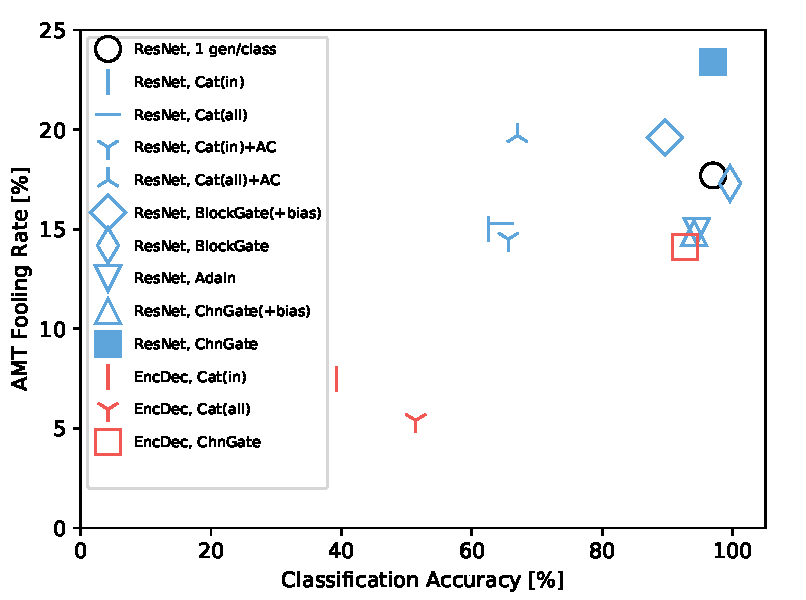
\includegraphics[width=\linewidth]{paper_images/gen_real_vs_acc.pdf}
%     \caption{Generation realism vs accuracy}\label{fig:conditioning_amt}
%     % \vspace{-4mm}
% \end{figure}

\begin{figure*}[t]%[ht!]
    \centering
    % \addSubFigHalf{gated_G_act}{Generator}{fig:gen_act} \addSubFigHalf{gated_D_act}{Discriminator}{fig:dis_act} 
    % \caption{Activation of the various blocks in the Generator and Discriminator}
    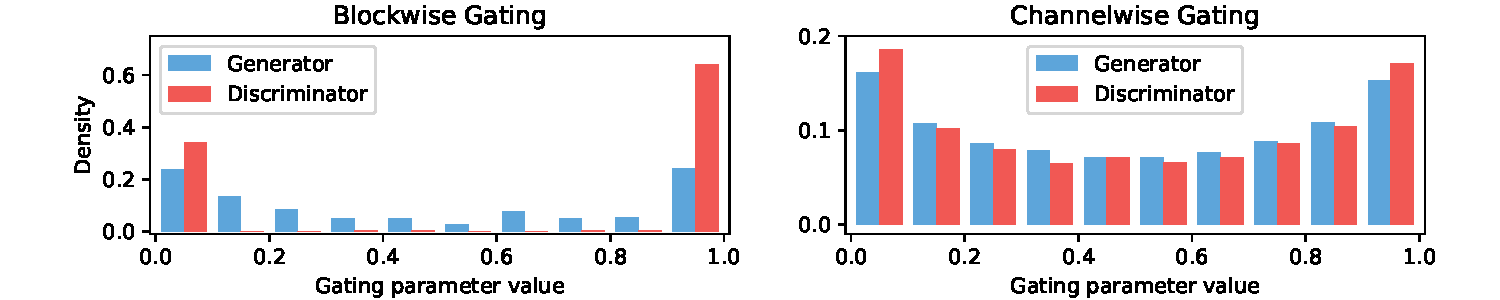
\includegraphics[width=\linewidth,trim={.7cm 0 .8cm 0},clip]{paper_images/alpha_hist.pdf}\caption{ {\bf Distribution of gating parameters.} We show the distribution of learned gating parameter $\alpha$ for {\bf (left)} blockwise and {\bf (right)} channelwise soft-gating. Values closer to 0,1 indicate that a residual block or channel is completely turned ``off" or ``on". In our best performing system, channelwise gating, the values are soft, but tend to be closer to the extremes.}
    \label{fig:alpha_dist}
    \vspace{-3mm}
\end{figure*}

% \paragraph{Network Architecture}
% \rz{shorten this into a few sentences for each net, so reader knows what we tested later, and point to suppmat where the tables can go}

% \subsection{Outline$\rightarrow$Image}
\subsection{Class-conditional image translation}

\noindent We further investigate the effect of soft-gating in image modeling scenarios. We first describe our dataset, which contains sparse inputs and is focused on multiclass generation. 

\noindent {\bf Dataset} Previous work~\cite{isola2016image2image,sangkloy2017scribbler,zhu2017unpaired,wang2017high} has trained edge-to-image translation. These systems have been post-hoc repurposed into a sketch-to-image translation machine, sometimes gaining unexpected popularity\footnote{Edges to cats demo: https://affinelayer.com/pixsrv/}. We collect 200 images (150 train, 50 test) for each of 10 classes -- basketball, chicken, cookie, cupcake, moon, orange, soccer, strawberry,  watermelon and pineapple -- and obtain rough outlines for each image. %using Adobe Photoshop
% Unlike previous work on scribble-to-image translation \cite{isola2016image2image,zhu2017unpaired,wang2017high},
Our outlines contain significantly less edge information. This makes the multitask generation problem more challenging -- for example, the same circular outline can draw a basketball, soccerball, or watermelon. A network must effectively integrate class information to be successful in this setting.
% , as the internal features must be learned by the network, and the same outline can generate substantially different images conditioned on different classes.
% , as seen in Fig.~\ref{fig:teaser}.
%The task involves multiple different objects of high realism when the input is very similar for the various classes several of them being exactly same(in the case of circular objects where the input scribble is an identical scribble for all circular classes). 

\noindent {\bf Network Architecture} Our preliminary experiments, using the architecture based on MUNIT~\cite{huang2018multimodal} did not succeed for this task. The architecture, which we refer to as {\bf Encoder-Decoder}, is comprised of 3 \texttt{conv} layers, 8 residual blocks, and 3 \texttt{up-conv} layers. The residual blocks have \rz{XXX} channels. We deepen the network, based on the principle that deeper networks have more valid disjoint, partially shared, paths~\cite{veit2016residual}, and add 26 residual blocks. To enable the larger number of residual blocks, we reduce the channels to 32 for every layer. Additionally, modifying the downsampling and upsampling blocks to be residual improved results, and also enables us to apply gating to {\em all} blocks. % , including the upsampling and downsampling residual blocks, improves the quality of generations. Additionally, we discover that even having few blocks  Details about the architecture can be found in the supplementary. \eli{explain why skinny.}
When gating is used, the gate prediction network, $\mathcal{F}$ in Fig.~\ref{fig:arch-gate} (mid-right, right) is also designed using residual blocks. We refer to this network as \textbf{SkinnyResNet}. Additional architectue details are in the supplementary material. 
We systematically test methods for injecting class information, as described in Sec.~\ref{sec:methods}. \begin{itemize}[noitemsep]
\item{\bf Per-class}: a single generator for each category; this is the only test setting with \textit{multiple} networks, all others train a single network
\item{\bf Concat (In)}: naive concatenation, input layer only
\item{\bf Concat (All)}: naive concatenation, all layers
\item{\bf Concat (In)+Aux-Class}: we add an auxiliary classifier, both for input-only and all layers settings
\item{\bf BlockGate(+Bias), BlockGate}: block-wise soft-gating, with and without a bias parameter
\item{\bf AdaIn}: Adaptive instance normalization
\item{\bf ChannelGate(+Bias), ChannelGate}: channel-wise soft-gating, with and without a bias parameter
\end{itemize}


% with each residual block consisting of 1D convolution layers. 

\begin{figure*}[h]
    \centering
    \includegraphics[width=.9\linewidth]{paper_images/cond_comp2.pdf}
    \caption{{\bf Algorithm Comparison:} Various Gating Mechanisms with our Skinny Resnet architecture succeeds in generating objects from respective classes which some of the baselines fail to do. The gating is not restricted to our skinny resnet architecture and can successfully be applied to the intermediate resnet blocks in an Encoder-Decoder architecture \cite{huang2018multimodal} \label{fig:alg_comp} }
    \vspace{-4mm}
\end{figure*}


% The incision experiments as performed by \cite{veit2016residual} showed that deeper networks have more  valid paths of computation. Our incision experiments on the 1D Mixture of Gaussians setting also demonstrated the effectiveness of having deeper residual networks with lesser number of neurons in each block. We therefore design a network architecture which doesn't change the number of channels even in the case where the spatial resolution changes since the gating is applied to all the blocks including the downsampling and upsampling residual blocks and the hypothesis is that the gating mechanism would work best if all the blocks had similar number of modulations per block.


\noindent \textbf{Evaluation Metrics} We evaluate the results on two important axes: adherence to conditioning and realism.

We first test the adherence to the conditioning -- whether the network generates an image of the correct class. Off-the-shelf networks have been previously used to evaluate colorizations~\cite{zhang2016colorful}, street scenes~\cite{isola2016image2image, wang2017high}, and ImageNet generations~\cite{salimans2016improved}. We take a similar approach and fine-tune a pretrained InceptionV3 network~\cite{szegedy2016rethinking} for our 10 classes. The generations are then tested with this network for classification accuracy.
% The class specific generations from the testset were passed through the finetuned network and the classifications were used to judge the class specific purity of the generations.

To judge the generation quality, we perform a ``Visual Turing test" using using Amazon Mechanical Turk (AMT). Turkers are shown a real image, followed by a generated image (or vice versa), and asked to identify the fake. An algorithm which generates a realistic image will ``fool" Turkers into choosing the the incorrect image. We use the implementation from~\cite{zhang2016colorful}. We show quantitative results in Fig.~\ref{fig:acc_vs_real} and qualitative examples in Fig.~\ref{fig:alg_comp}.

\paragraph{Does naive concatenation effectively inject conditioning?} In Fig.~\ref{fig:alg_comp}, we show a selected example from each of the 10 classes. The per-class baseline trivially adheres to the conditioning, as each class gets to have its own network. However, when a single network is trained to generate all classes, naive concatenation is unable to successfully inject class information, for either network and for either type of concatenation. For the \textbf{EncoderDecoder} network, basketballs, oranges, cupcakes, pineapples, and fried chicken are all confused with each other. For the \textbf{SkinnyResNet} network, oranges are generated instead of basketballs, and pineapples and fried chicken drumsticks are confused. As seen in Fig.~\ref{fig:acc_vs_real}, classification accuracy is slightly higher when concatenating all layers versus only the input layer, but is low for both ($62.6\%$ and $64.5\%$).
% As evident from \figref{fig:alg_comp} for some classes naive concatenation helps in generating appealing images but for some classes it either fails to generate images from the right class or generates unrealistic images from that class.
% No, point to Figure 9 (qualitative grid) \& Figure 10 (the plot)

% \paragraph{Does gating produce accurate and realistic conditional generations?} The gating mechanisms succeeds in generating realistic images from each class while also preserving the class conditioning appropriately. As evident from the comparisons of generations in \figref{fig:alg_comp} and the metrics reported in \figref{fig:conditioning_amt} the channel wise multiplication produces the most visually appealing results amongst the various gating mechanisms.
% Yes, point to Figure 9 results. Also analyze which variation is the best

\paragraph{Does gating effectively inject conditioning?} Using the proposed soft-gating, on the other hand, leads to succesful generations. We test variants of soft-gating on the \textbf{SkinnyResNet}, and accuracy is dramatically improved, between $89.6\%$ to $99.6\%$. Among the gating mechanisms, we find that channel-wise multiplication
% (on both generator and discriminator)
generates the most realistic images, and achieves an AMT fooling rate of $23.4\%$. Interestingly, the fooling rate is higher than the per-class generator of $17.7\%$. Qualitatively, we notice that per-class generators sometimes exhibits artifacts in the background, as seen in the generation of "moon". We hypothesize that the single generator with gating has the benefit of seeing more training data and finding common elements across those classes, such as clean, white backgrounds.
% The classification accuracy of an Inception network finetuned on our dataset demonstrates the purity of the generations corresponding to the correct class using the gating mechanism. 

% As seen in \figref{fig:alg_comp}, all of the various gating mechanisms and the baselines are able to generate images of high quality and realism from some classes but most of the baselines fail in some classes, often mixing visual features from wrong classes. 


\begin{figure*}[h]
    \centering
    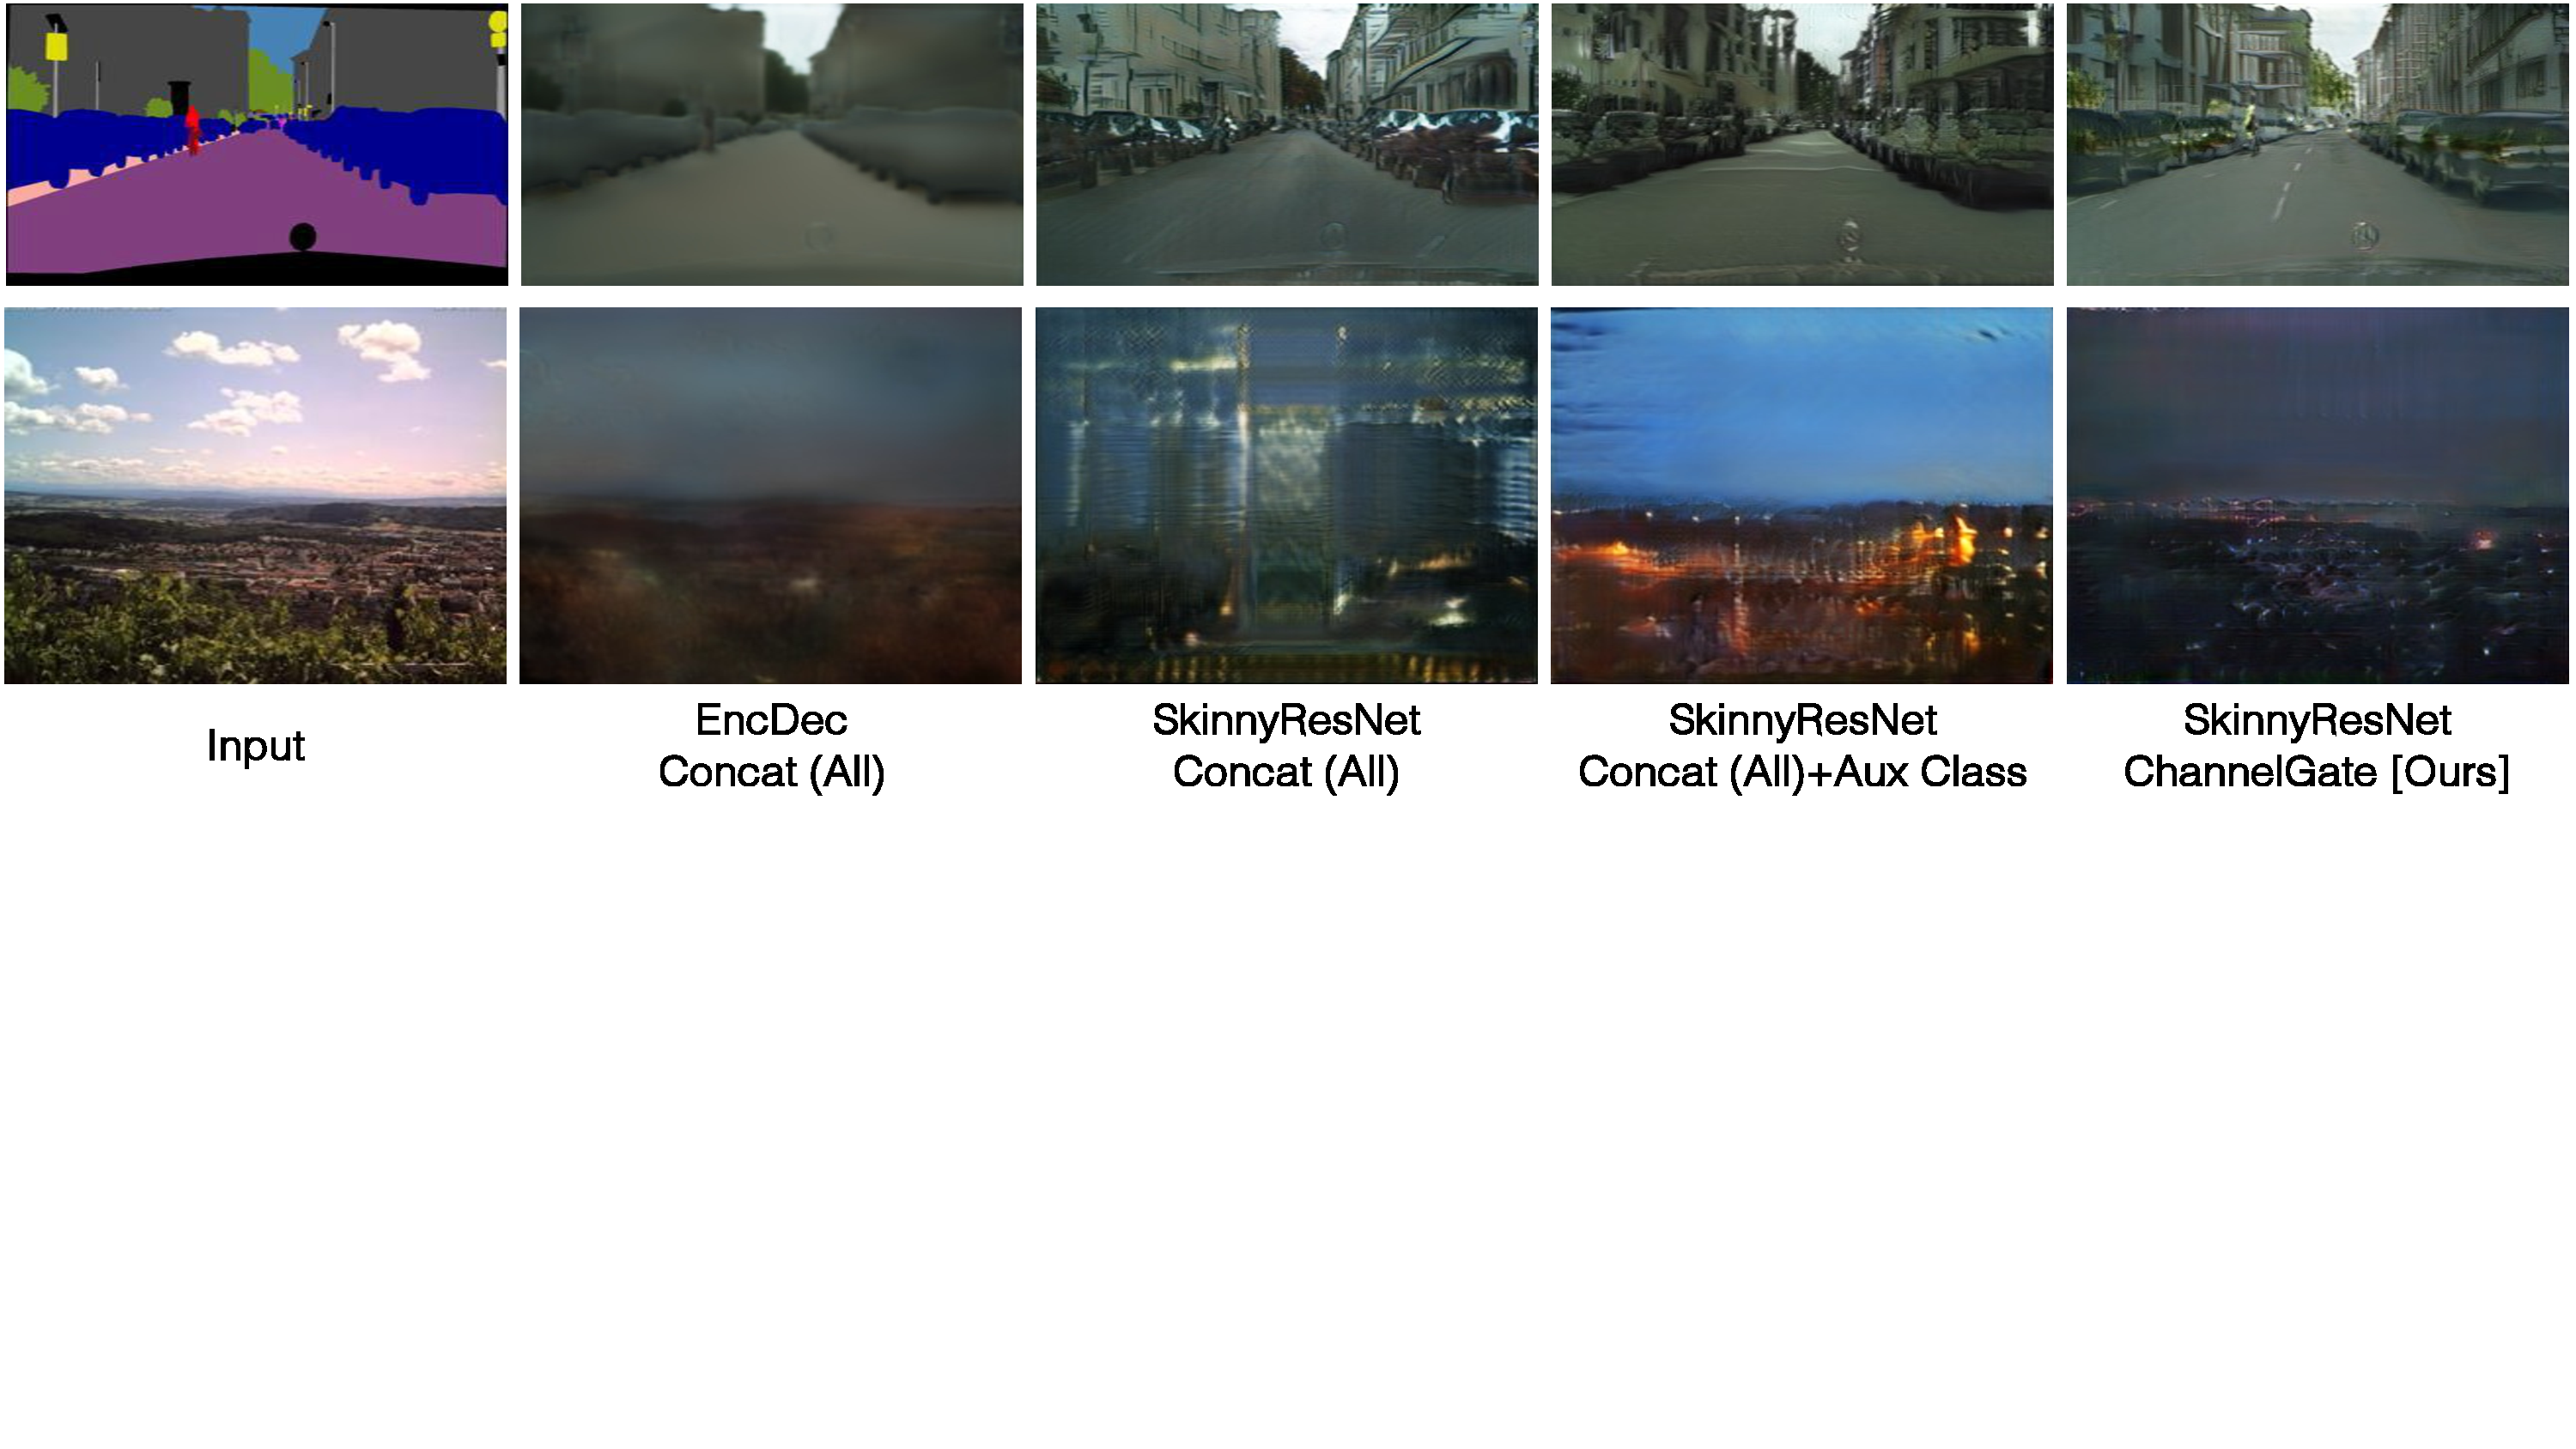
\includegraphics[width=1.\linewidth]{paper_images/multitask_comp.pdf}
    \caption{\textbf{Multitask generation results}. Single network trained on both Cityscapes Label$\rightarrow$Image and Day$\rightarrow$night. The proposed channelwise gating method (right) is able to better incorporate task conditioning and produces more realistic results.
    % \ow{seems like this is missing 1. two generators, and 2. one generator. instead it seems more like an ablation study on our method, which is not the point. would be more impressive to show it matches 2 generators and 1 generator totally fails.}
    }
    \label{fig:multi-task_day2night}
    \vspace{-2mm}
\end{figure*}

\begin{table*}[t]
  \floatsetup{floatrowsep=qquad, captionskip=4pt}
  \centering
    \begin{floatrow}[2]
    \ffigbox[\FBwidth]{
    \scalebox{0.95} {
        \begin{tabular}{l c}
        % \hline
        \toprule
        \textbf{Model} & \textbf{LPIPS Distance} \\ \midrule
        Random Real Images & $0.3665 \pm 0.0053$ \\ \midrule
        BicycleGAN~\cite{zhu2017toward} & $0.1374 \pm 0.0005$  \\ \midrule
        Concat(In) &  $0.0432 \pm 0.0002$ \\
        Concat(All) & $0.0159 \pm 0.0004$ \\ \cdashline{1-2}
        ChannelGate [Ours] & $0.0964 \pm 0.0003$  \\
        \bottomrule %inserts single line
        \end{tabular}}}
        {\caption{\label{table:infogan_lpips} {\bf Edges$\rightarrow$Handbags Diversity} We measure LPIPSv0.1~\cite{zhang2018unreasonable} distance between randomly generated handbags, given the same edge map, as proposed in~\cite{zhu2016generative}. Given the same architecture, gating achieves higher diversity than concatenation.}}
        \ffigbox[\FBwidth]{
        \scalebox{0.95} {
        \begin{tabular}{l c c c} % 
        % \begin{tabular}{p{6cm}c{1.8cm}c{1.8cm}c{1.8cm}} % centered columns (4 columns)
        \toprule
        \multirow{2}{*}{\textbf{Model}} & \textbf{Per-pixel} &  \textbf{Per-class } & \textbf{Class} \\
        & \textbf{Acc} &  \textbf{Acc} & \textbf{IOU} \\ \midrule
        Pix2pix \cite{isola2016image2image} & 0.660  & 0.23 & 0.17 \\ \midrule
        EncDec, Concat(All) & 0.600 & 0.16 & 0.15 \\ \cdashline{1-4}
        SkinnyResNet, Cat(All) & 0.602 & 0.18 & 0.16 \\
        SkinnyResNet, Cat(All)+Aux-Class & 0.675 & 0.20 & 0.16 \\ \cdashline{1-4}
        SkinnyResNet, ChannelGate [Ours] & 0.684 & 0.23 & 0.18 \\ \bottomrule
        % \bottomrule %inserts single line
        \end{tabular}}}{
        \caption{ {\bf Cityscapes generation accuracy}. We evaluate the accuracy of Cityscapes Label$\rightarrow$Image generation results, as part of the multitask test. The network is also trained for an unrelated Day$\rightarrow$Night task. A pre-trained segmentation network~\cite{XX} evaluates the synthesized results. Gating achieves higher results than concatenation, as well as single-task pix2pix~\cite{isola2016image2image}.}
        \label{label:me}}
    
  \end{floatrow}
%  \vspace{-2mm}
%   \label{fig:real_vs_div}
\end{table*}


% \begin{figure}
%     \centering
%     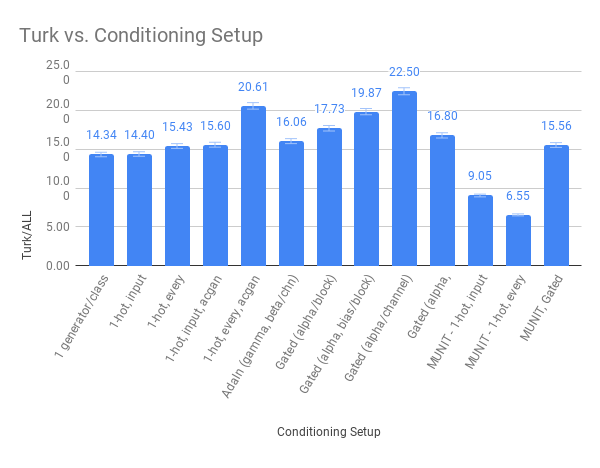
\includegraphics[width=\linewidth]{conditioning_amt.png}
%     \caption{AMT studies of the various gating techniques on the scribble dataset}\label{fig:conditioning_amt}
%     \vspace{-4mm}
% \end{figure}

\begin{figure}[t]
    \centering
    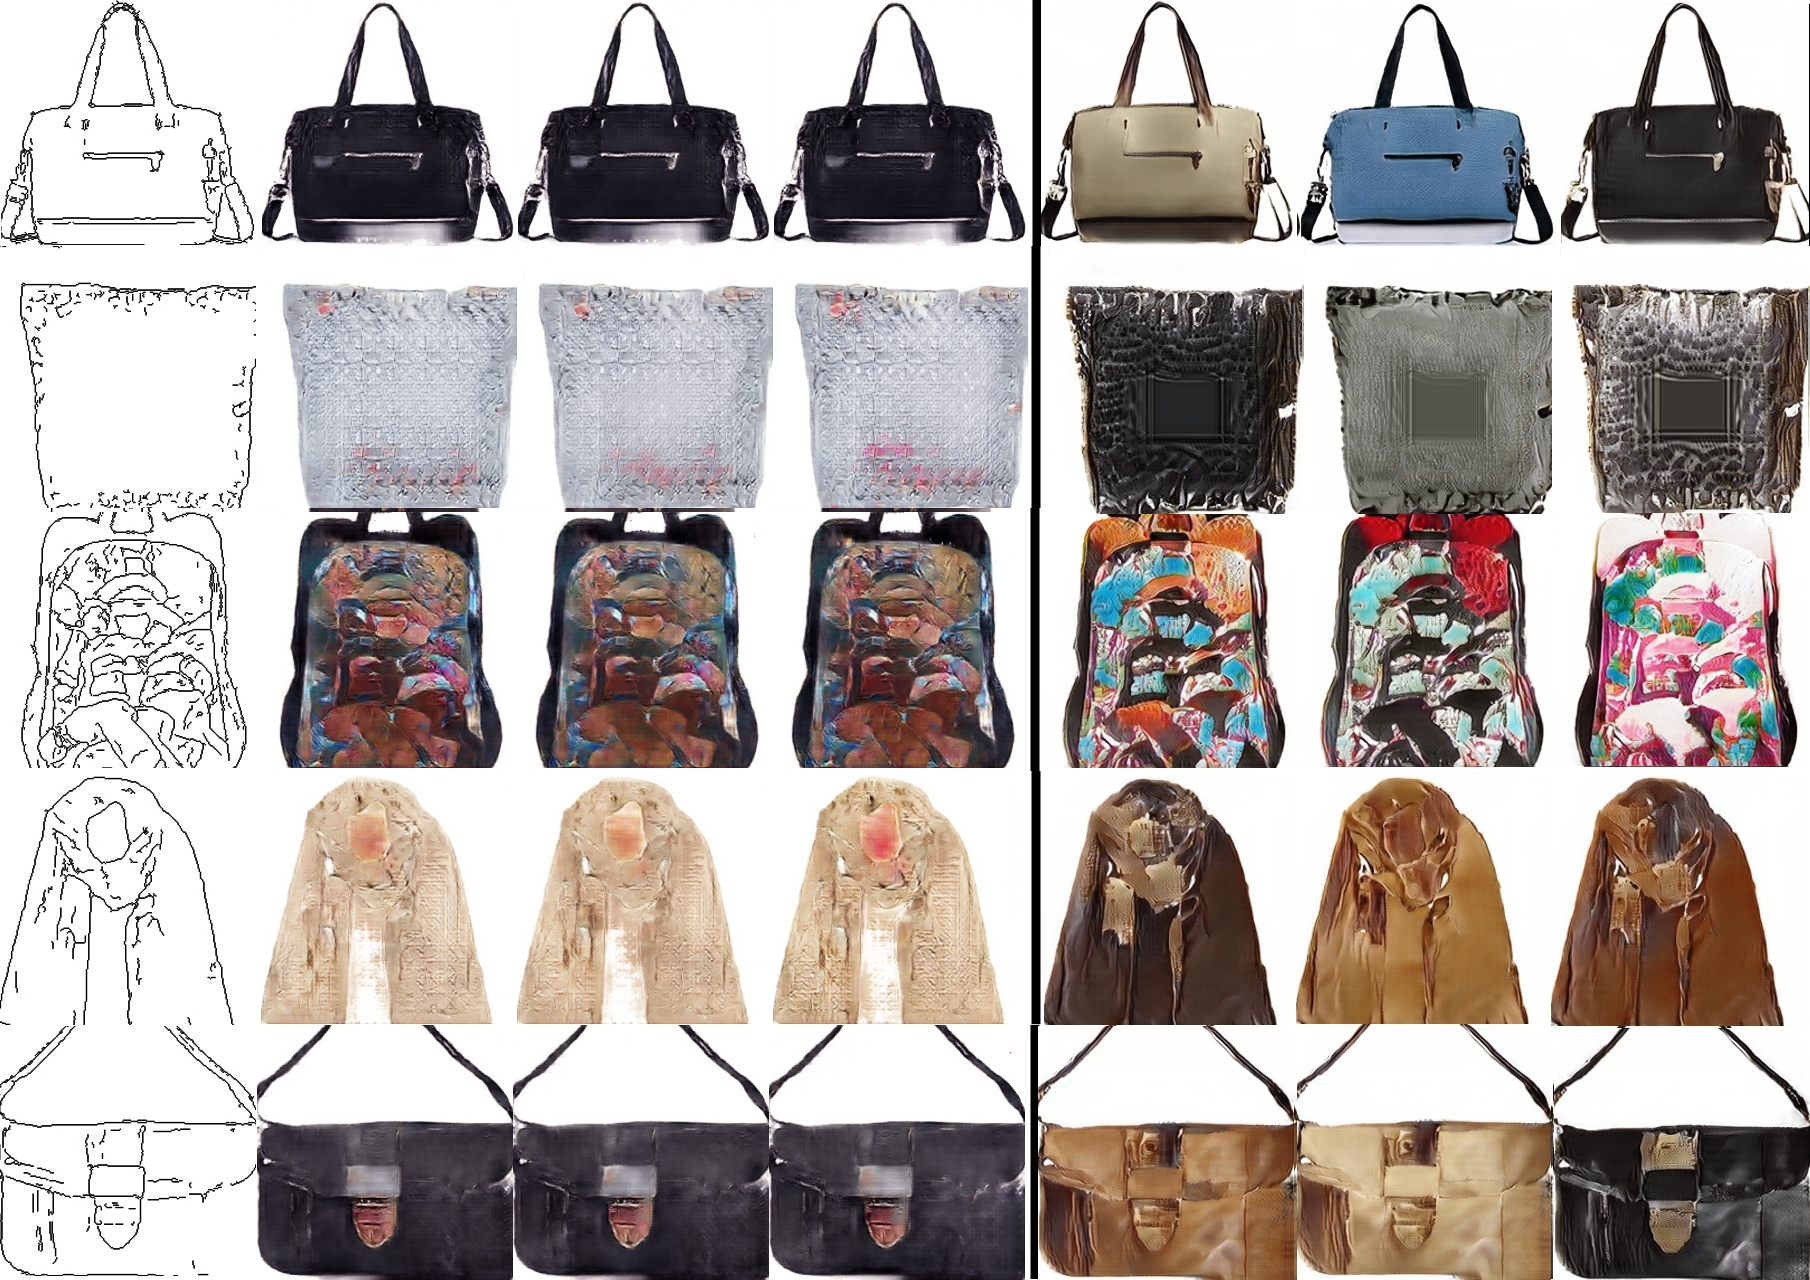
\includegraphics[width=\linewidth]{infogan.jpg}
    \caption{{\bf Edges$\rightarrow$Handbags qualitative examples.} Naive Conditioning of InfoGAN fails (left) while gating (right) succeeds in producing diverse generations.}\label{fig:infogan_gate}
    \vspace{-2mm}
\end{figure}

\noindent \textbf{Is gating effective across architectures?} 
% We evaluate the following architectures on the outlines-to-images task. 
% We first evaluate our \todo{SkinnyResNet} with a more traditional encoder-decoder architecture. 
% We use the architecture proposed in MUNIT~\cite{huang2018multimodal} which consists of an encoder followed by a set of residual blocks with a decoder at the end.
As seen in Fig.~\ref{fig:acc_vs_real}, using channelwise gating instead of naive concatenation improves performance both accuracy and realism \textit{across} architectures. For example, for the \textbf{EncoderDecoder} architecture, gating enables successful generation of the pineapple.
% In this case, we apply the gating to this architecture only on the bottleneck residual blocks.
% As evident from \figref{fig:alg_comp} although the network learns to disentangle the various classes, the generation quality reduces from the skinny resnet architecture where all the layers are gated.
Both quantitatively and qualitatively, results are better for our proposed \textbf{SkinnyResNet} architecture.

% Yes, works for both skinny resnet \& enc-dec.

\paragraph{Do the generations generalize to unusual outlines?} The training images consist of the outlines corresponding to the accurate geometry for each class. However, an interesting test scenario is whether the technique generalizes to unseen shape and class combinations. In \figref{fig:teaser}, we show that an input circle and not only produce circular objects, such as a basketball, watermelon, and cookie, but also noncircular objects such as strawberry, pineapple, and cupcake. Note that both the pineapple crown and bottom are generated, even without any structural indication of these parts in the outline.

\paragraph{How are the gating coefficients distributed?} In Fig.~\ref{fig:alpha_dist}, we show the distribution of predicted gating parameters, for both blockwise and channelwise gating. The parameters tend to be closer to 0, for ``off" and 1, for ``on". For blockwise gating, the discriminator is almost completely binary. For channelwise gating, the discriminator tends slightly more to the extremes than the generator.
% An interesting observation of the gating coefficients in the case of the block wise gating mechanism, as demonstrated in \figref{fig:gated_block_act} for different classes different sets of blocks were activated and some blocks were totally deactivated for some classes. The switching on and off of various blocks without even adding a sparsity constraint was better defined in the case of the discriminator.


% \begin{figure*}[h]
%     \centering
%     \includegraphics[width=.94\linewidth]{paper_images/cond_comp2.pdf}
%     \caption{{\bf Algorithm Comparison} \label{fig:alg_comp} }
%     \vspace{-4mm}
% \end{figure*}



% \begin{figure}
%     \centering
%     \includegraphics[width=\linewidth]{paper_images/cond_comp.pdf}
%     \caption{Algorithm Comparison}\label{fig:conditioning_amt}
% \end{figure}

% In the widely popular image conditioned generative models introduced in Pix2pix by \cite{isola2016image2image} although the results are brilliant, it had the inherent problem of only being applicable to a particular task such as different networks had to be trained for edges to shoes and edges to handbags, although StarGAN \cite{choi2017stargan} mitigated some of the problems but it was only applicable for relatively minute transformations such as changing the characteristics of the face.

% To analyze properly the task of multi-class generations in the image conditioned setting we introduce a new task of generating class conditioned realistic images from very rough scribbles. We start off with 3 classes, namely: pizza, strawberry and oranges. A simple pix2pix network fails to identify the different classes and starts injecting weird textures such as pizza on orange or strawberry on pizza as depicted in the results from pix2pix on this task in \figref{fig:scribble_pix2pix}. 

% In the conditional setting for the generator, the main block only receives the input scribble and the gate selection block receives the class condition and predicts the $aplha^i$s for the gated residual blocks. The discriminator on the other hand is composed of a main network consisting of gated residual blocks which is oblivious to the class conditioning and a gate selection network which predicts the $aplha^i$s for the main network of the discriminator. The main network also receives the input scribble alongside the generated/real image to predict how real/fake an image is based on the alpha weightings of its gated residual blocks. The network is able to disentangle the class conditioning although none of the main networks of the generator/ discriminator are aware of the class conditioning, the class information only being input to the gate selection network which has to modulate the weights of the respective networks' gated residual blocks. The results of the model are depicted in \figref{fig:scribble_grb} whereby we can clearly see that the network has been able to disentangle the class conditioning and generate textures appropriate for the right class.


% \subsection{Comparison to other forms of conditioning in Resblock :}
% Conditional Batch Normalization, FiLM and Adaptive Instance Normalization are the techniques which are the most closely related to our methodology. All of these have the benefit of being applicable even without the presence of residual blocks in the architecture. So an exhaustive comparison with all of these methods along with our form of conditioning on the residual blocks is a valid set of experimentation and has to be done to make the paper complete.

% \subsection{Infogan Variations(pix2pix):}
\subsection{Edges $\rightarrow$ Handbags (Multimodal Generations)}
Inter-class variation, also called diversity, is a significant challenge in GAN image generation applications. 
In the pix2pix setting, as shown by previous works \cite{ghosh2017multi} and \cite{zhu2017toward} even the InfoGAN (cLR in \cite{zhu2017toward}) setup was not able to produce meaningful variations in the generations, or needed multiple generators or cyclical losses to produce meaningful variations in the generated images. 
With our gating mechanism, we show that we can create meaningful variations in the generated samples conditioned on a single sketch as evident from the generations \figref{fig:infogan_gate} and from the LPIPS metric \cite{zhang2018unreasonable} in  Table. \ref{table:infogan_lpips} which measures the diversity among the generations in the feature space of a standard Imagenet classifier.
\ow{needs more detail}




% \begin{table}[ht]
% \caption{Evaluation on Edges to Handbags diverse generations. Diversity using LPIPS metric \cite{zhang2018unreasonable}} % title of Table
% \small
% \centering % used for centering table
% % \begin{tabular}{|c|c|c|c|} % centered columns (4 columns)
% \begin{tabular}{p{3cm}p{3cm}} % centered columns (4 columns)
% % \hline
% \toprule
% \textbf{Model} & \textbf{LPIPS Distance} \\%heading
% \midrule
% BicycleGAN \cite{zhu2017toward} & $0.1374 \pm 0.0005$  \\ % inserting body of the table
% \midrule
% Ours(Gated) & $0.0964 \pm 0.0003$  \\
% \midrule
% Concat(Input) &  $0.0432 \pm 0.0002$ \\
% \midrule
% Concat(All Layers) & $0.0159 \pm 0.0004$ \\
% \midrule
% Random Real Images & $0.3665 \pm 0.0053$ \\
% \bottomrule %inserts single line
% \end{tabular}
% \label{table:infogan_lpips} % is used to refer this table in the text
% \end{table}

% \begin{figure*}[t]%[ht!]
% \centering
% \begin{tabular}{*{5}{c@{\hspace{3px}}}}
%     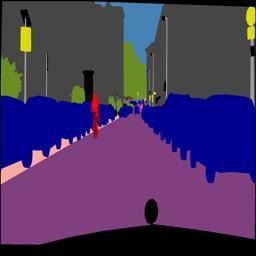
\includegraphics[width=.18\linewidth]{channel_gated/cityscapes_95_real_A} &
%     \includegraphics[width=.18\linewidth]{munit_baseline_all/cityscapes_95_fake_B} &
%     \includegraphics[width=.18\linewidth]{our_baseline_all/cityscapes_95_fake_B} & 
%     \includegraphics[width=.18\linewidth]{acgan_baseline_all/cityscapes_95_fake_B}&
%     \includegraphics[width=.18\linewidth]{channel_gated/cityscapes_95_fake_B} \\
    
%     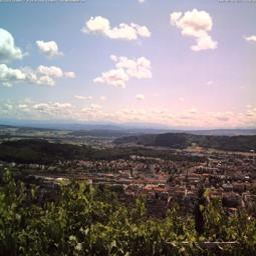
\includegraphics[width=.18\linewidth]{final_images/channel_gated/night2day_35_3106_to_3109_real_A.jpg} &
%     \includegraphics[width=.18\linewidth]{munit_baseline_all/night2day_35_3106_to_3109_fake_B} &
%     \includegraphics[width=.18\linewidth]{our_baseline_all/night2day_35_3106_to_3109_fake_B} &
%     \includegraphics[width=.18\linewidth]{acgan_baseline_all/night2day_35_3106_to_3109_fake_B} & 
%     \includegraphics[width=.18\linewidth]{channel_gated/night2day_35_3106_to_3109_fake_B}\\
    
%     \begin{subfigure}[t]{.18\linewidth}\caption{\small Input}\label{fig:daynightinput}\end{subfigure} &
%     \begin{subfigure}[t]{.18\linewidth}\caption{\small Enc-Dec Concat (All)}\label{fig:daynightinput}\end{subfigure} &
%     \begin{subfigure}[t]{.18\linewidth}\caption{\small Concat (All)}\label{fig:daynightinput}\end{subfigure} &
%     \begin{subfigure}[t]{.18\linewidth}\caption{\small Concat(All)+Aux-Class}\label{fig:daynightinput}\end{subfigure} &
%     \begin{subfigure}[t]{.18\linewidth}\caption{\small Ours}\label{fig:daynightinput}\end{subfigure}\\
% \end{tabular}
%     % \addSubFigEighth{channel_gated/cityscapes_95_real_A}{input}{fig:city_input} 
%     % \addSubFigEighth{channel_gated/cityscapes_95_fake_B}{Ours}{fig:city_ours} 
%     % \addSubFigEighth{munit_baseline_all/cityscapes_95_fake_B}{MUNIT Conditioning all layers}{fig:city_munit}
%     % \addSubFigEighth{our_baseline_all/cityscapes_95_fake_B}{Our Architecture Conditioning all layers}{fig:bag_3}
%     % \addSubFigEighth{acgan_baseline_all/cityscapes_95_fake_B}{ACAN (our Architecture Conditioning all layers) }{fig:bag_3}
%     % \caption{Various Methods for Cityscapes for Multi-Task Experiment}
%     % \label{fig:multi-task_cityscapes}
%     % \vspace{-3mm}
%     % \addSubFigEighth{channel_gated/night2day_58_5018_to_5000_real_A}{input}{fig:city_input} 
%     % \addSubFigEighth{channel_gated/night2day_58_5018_to_5000_fake_B}{Ours}{fig:city_ours} 
%     % \addSubFigEighth{munit_baseline_all/night2day_58_5018_to_5000_fake_B}{MUNIT Conditioning all layers}{fig:city_munit}
%     % \addSubFigEighth{our_baseline_all/night2day_58_5018_to_5000_fake_B}{Our Architecture Conditioning all layers}{fig:bag_3}
%     % \addSubFigEighth{acgan_baseline_all/night2day_58_5018_to_5000_fake_B}{ACAN (our Architecture Conditioning all layers) }{fig:bag_3}
%     \caption{Results on the multi-task generation problem with Segmentation2Cityscapes and Day2Night. \ow{seems like this is missing 1. two generators, and 2. one generator. instead it seems more like an ablation study on our method, which is not the point. would be more impressive to show it matches 2 generators and 1 generator totally fails.}}
%     \label{fig:multi-task_day2night}
%     \vspace{-3mm}
% \end{figure*}


% \begin{table}[ht]
% \caption{Evaluation on Cityscapes for Multi-Task scenario. A pre-trained segmentation network~\cite{} performs a semantic segmentation on generated images, and the result is compared to the ground truth.} % title of Table
% \small
% \centering % used for centering table
% % \begin{tabular}{|c|c|c|c|} % centered columns (4 columns)
% \begin{tabular}{p{3cm}p{1cm}p{1cm}p{1cm}} % centered columns (4 columns)
% % \hline
% \toprule
% \textbf{Model} & \textbf{Per-pixel acc.} &  \textbf{Per-class acc.} & \textbf{Class IOU} \\%heading
% \midrule
% Pix2pix \cite{isola2016image2image} & 66 \%  & 0.23 & 0.17 \\ % inserting body of the table
% \midrule
% Ours(Channel-Gate) & 68.4 \%  & 0.23 & 0.18 \\
% \midrule
% Concat(All),Aux-class & 67.5 \% & 0.2 & 0.16 \\
% \midrule
% Concat(All) & 60.2 \% & 0.18 & 0.16 \\
% \midrule
% Enc-Dec, Concat(All) & 60 \% & 0.16 & 0.15 \\
% \bottomrule %inserts single line
% \end{tabular}
% \label{table:1d_G} % is used to refer this table in the text
% \end{table}

\subsection{Multi-Task Generation }
We also evaluate two previously shown image-to-image translation tasks, using the {\em same} network. 
%Since our network is robust enough to be able to generate images conditioned on class and modulation of which blocks to use, it can further be used to generate images which are different in tasks such as the same network
We try to solve both segmentation map $\rightarrow$ street scene, and day $\rightarrow$ night image translation tasks using the same generator. 
As we can see in \figref{fig:multi-task_day2night}, our model (Channel-Gate) is able to perform both tasks while the other techniques generate mixed results. 

In case of Encoder-Decoder architecture \cite{huang2018multimodal} conditioned on all layers, the discriminator became too powerful after a while and the training progressed with only the L1 loss which caused the blurry generations in the case of segmentation maps to real image synthesis as evident from the figure. The other baselines based on our \todo{SkinnyResNet} architecture failed to generate realistic images in the case of the task of day2night.



% \section{Planned Set of Experiments:}
% \subsection{Unconditional Generations :}
% Since the model is not restricted to be applicable only in the image to image setting and is more general than that, if we get the unconditional generations working at least on the places dataset and the faces(it also has got some class labels that can be used for conditioned generation). It will be a good generalization. A bit of engineering might be required to get the architecture working on the unconditional case since the structure of the generator and discriminator would be different from the current generator which takes an image as an input and outputs an image of the same resolution. The discriminator in the case of the current image2image experiments employ a patch based discriminator which has to be modified to work in the unconditional generation setting.




% \subsection{Instance Based Generations: }
% As demonstrated by the early experiments I performed with pix2pixhd that it overfits the dataset and simplification of the same instance map led to garbled generations showed that it was unstable to perturbations. Instance based generations could be possible with our model since we already know which pixels are for which class and we can generate instances of each class separately and then stitch together the various class generations into a final image.


% \section{Directions about novelty of approach:} 

% \subsection{Learning to Learn}
% Learning to learn is becoming an increasingly relevant paradigm for deep learning models as the power of the networks increase and we want less hyper parameter tuning. Our model can be perceived as a system whereby the hypernetwork responsible for predicting the $\alpha_i$ of each block is learning by analyzing the function learnt by each block and thereby distributing the blocks between the various different classes for the generator and the discriminator. We will have to look deeply into the literature to identify the connections with the learning to learn paradigm.

% \subsection{Ensembles of several shallower nets (implicit MAD-GAN)}
% The initial motivation of Eli and Oliver was to extend MAD-GAN with the intuitions gained by Andreas Veit's paper on Residual Blocks acting as ensembles of several shallower networks. The structure of the paper at the moment follows that intuition and the experiments on the 1D Mixture of Gaussians demonstrates that residual blocks indeed behave as ensembles of several shallower networks even in the case of generative models.

% \subsection{Effective way of fusing high dimensional and low dimensional information}
% The techniques proposed in this paper provides a way of effectively fusing high dimensional information in the form of images and low dimensional conditioning in terms of class conditioning or sampled conditioning as in the form of InfoGAN. Further the multi-task application demonstrates the efficacy of the fusing of task information alongside the high dimensional information about images.





\section{Conclusion}
\noindent In conclusion, we have presented an evaluation of different gating mechanisms to allow for multiclass image generation using GANs. 
We propose an auxiliary channelwise gating network for conditioning combined with a skinny ResNet, and show that this combination improves state-of-the-art results in both class-conditioned and unsupervised settings.

%Its interesting to observe that with a simple residual block on the non-parametric density estimation task, the removal of certain blocks corresponds to the removal of modes in the generated distribution and the incision of different blocks corresponding to the removal of the same mode from the generated distribution shows the validity of the claims in \cite{veit2016residual} which says that residual networks behave as an ensemble of several shallower networks. 

%The results with the Gated Residual Blocks on the Generator on the infoGAN configuration for unconditional setting and the image conditional setting proves the efficacy of the gated residual blocks on the respective tasks. The results of the Gated Residual Blocks on the side of the discriminator shows an intriguing observation that inspite the network being oblivious of the class conditioning, the gate selection network aptly distributed the right blocks for the appropriate classes to disentangle the class conditioning. The Gated Residual Blocks has applications beyond GANs and can be used potentially in many conditional scenarios such as text to image synthesis or Conditional Variational Autoencoders. 

% \section{Conclusion}
% The paper introduced a novel model to disentangle image information and low dimensional information using Gated Residual Blocks which was efficient in generating images in the unconditional setting for infoGAN as well as class and image conditioned setting for the pix2pix variant. The paper also introduced the novel task of class conditional realistic image synthesis from rough scribbles, in which the proposed model performed quite favorably.


{\small
\bibliographystyle{ieee}
\bibliography{src/gatedblocks}
}


\section*{Supplemental material}


\subsection{InfoGAN based Model}
The intuitions gained from the experiments performed for the non-parametric density estimation led to the Gated Residual Block on the Generator of a GAN. InfoGAN \cite{chen2016infogan} presented a perfect setting to apply the Gated Residual Block in the case of the generator. The first set of experiments were on MNIST and Fashion-MNIST with sets of 10 discrete variables (since there were 10 classes in both of the datasets) and 2 continuous variables whose information was tried to be maximized using the Q network. As can be seen in \figref{fig:infogan_unconditional} the network was able to generate realistic images from the different classes and produce meaningful interpolations by varying the continuous variables as shown in the figure. The exact experimental setting was that the hypernetwork responsible for the predictions of the $alpha^i$s which we term as the gate selection network gets the salient variables and has no information about the random noise sampled for the main network(consisting of gated residual blocks), based on the salient variables received the gate selection network predicts the  $alpha^i$s for all the blocks of the network. The main network is oblivious of the conditioning received in the salient variables and has to generate images coherent with the conditioning since the Q-Network tries to reconstruct back the conditioning received in the form of salient variables. 

\begin{figure}[t]%[ht!]
    \centering
    \addSubFigHalf{Picture35}{MNIST}{fig:infogan_mnist} 
    \addSubFigHalf{Picture34}{Fashion-MNIST}{fig:infogan_fashion_mnist} 
    \caption{Gated Residual Block-InfoGAN on MNIST and Fashion MNIST \ow{do we have the standard infogan comparison here?}}
    \label{fig:infogan_unconditional}
    \vspace{-3mm}
\end{figure}

\subsection{Unconditional Generations}
\begin{figure}[t]
    \centering
    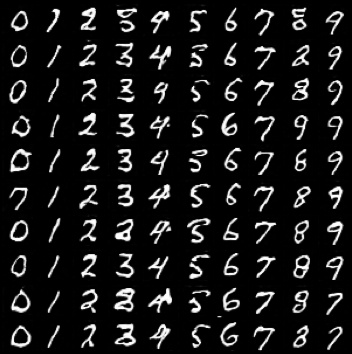
\includegraphics[width=0.5\linewidth]{Picture5}
    \caption{Results on the Gated Residual Block on MNIST dataset}\label{fig:grb_mnist}
    \vspace{-4mm}
\end{figure}

A well known problem in image conditional GAN settings is the tendency to produce realistic outputs but not being able to produce meaningful variations in the generated output. It was especially prevalent in the original pix2pix setting \cite{isola2016image2image} and further research enabled variations such as \cite{ghosh2017multi} and \cite{zhu2017toward}. Although as shown in \cite{ghosh2017multi} the naive infoGAN setting couldn't produce meaningful variations in the pix2pix setting, settling rather for very minute variations. Our Gated Residual Blocks could mitigate some of the problems and did produce variations in the challenging task of edges-to-bag generation as has been demonstrated in \figref{fig:infogan_bags}. By varying the continuous variable smooth interpolations could be obtained between colors and textures which was earlier not possible with the infogan based pix2pix setting. Although the variations along the discrete axis was quite minimal and we are still investigating the cause for the same. The experimental setting in this scenario was that the salient variables were only given to the gate selection network and had to predict the $alpha^i$s for the main network which consisted of gated residual blocks and was oblivious of the conditioning provided in the form of salient variables. The Discriminator network was the standard image conditional discriminator network while the Q network in this scenario was modified to take the generated image as well as the edge map to behave as a image conditional Q Network which tries to reconstruct back the salient variables given to the gate selection network. 

\newcommand{\addSubFigEighth}[3]{\begin{subfigure}[t]{.18\linewidth}
   \includegraphics[width=\linewidth]{#1}
   \caption{#2}\label{#3}\end{subfigure}
}
\newcommand{\addSubFigEighthCaptionless}[3]{\begin{subfigure}[t]{.18\linewidth}
   \includegraphics[width=\linewidth]{#1}
   \label{#2}\end{subfigure}
}

The next set of experiments were performed to judge the robustness of the Gate Selection Blocks and the Gated Residual Blocks in the case the labels were available. That meant using the gate selection network and the gated residual blocks on the discriminator. The implications were even more interesting, the gate selection network would have to distribute the blocks between the classes to get the class specific gradients back for training the class conditioned generator. In the unconditional setting for the generator, the main block only receives random noise and the gate selection block receives the class condition and predicts the $aplha^i$s for the gated residual blocks. The discriminator on the other hand is composed of a main network consisting of gated residual blocks which is oblivious to the class conditioning and a gate selection network which predicts the $aplha^i$s for the main network of the discriminator. The main network predicts how real/fake an image is based on the alpha weightings of its gated residual blocks. The network is able to disentangle the class conditioning although none of the main networks of the generator/ discriminator are aware of the class conditioning, the class information only being input to the gate selection network which has to modulate the weights of the respective networks' gated residual blocks. The generated samples on the MNIST dataset are shown in \figref{fig:grb_mnist} and the alpha gatings for the different classes and the different blocks in \figref{fig:mnist_act}. The values for the gates clearly show switching off of certain blocks in the case it is not needed for a particular class even though a sparsity constraint was not applied in the training objective.


\begin{figure}%[ht!]
    \centering
    \addSubFigHalf{Picture6}{Activations of the gated residual blocks in the generator}{fig:gen_act} 
    \addSubFigHalf{Picture7}{Activations of the gated residual blocks in the discriminator}{fig:dis_act} 
    \caption{Activation of the various blocks in the Generator and Discriminator}
    \label{fig:mnist_act}
    \vspace{-3mm}
\end{figure}






\begin{figure*}[t]%[ht!]
    \centering
    \addSubFigEighthCaptionless{Picture8}{Sketch}{fig:bag_sketch} 
    \addSubFigEighthCaptionless{Picture9}{Varition 1}{fig:bag_1} 
    \addSubFigEighthCaptionless{Picture10}{Varition 2}{fig:bag_2}
    \addSubFigEighthCaptionless{Picture11}{Varition 3}{fig:bag_3}
    \addSubFigEighthCaptionless{Picture12}{Varition 4}{fig:bag_4}
    \caption{The variations produced in the sketch to realistic bag task in the infogan with Gated Residual Block setting for the generator }
    \label{fig:infogan_bags}
    \vspace{-3mm}
\end{figure*}




\subsection{1-D network architecture}

\begin{table}[ht]
\caption{Resblock} % title of Table
\centering % used for centering table
\begin{tabular}{c} % centered columns (4 columns)
\hline\hline %inserts double horizontal lines
F(x)\\%heading
\hline % inserts single horizontal line
Linear(nneurons,nneurons)\\ % inserting body of the table
ReLU() \\
Linear(nneurons,nneurons) \\
\hline %inserts single line
\end{tabular}
\label{table:resblock} % is used to refer this table in the text
\end{table}


\begin{table}[ht]
\caption{\textbf{Generator for 1D setting}} % title of Table
\centering % used for centering table
\begin{tabular}{c c} % centered columns (4 columns)
\hline\hline %inserts double horizontal lines
layer & num layers\\%heading
\hline % inserts single horizontal line
Linear(10,4) & 1\\ % inserting body of the table
ResBlock(4) & 16 \\
Linear(4,1) & 1 \\
\hline %inserts single line
\end{tabular}
\label{table:1d_G} % is used to refer this table in the text
\end{table}

\begin{table}[ht]
\caption{\textbf{Discriminator for 1D setting}} % title of Table
\centering % used for centering table
\begin{tabular}{c c} % centered columns (4 columns)
\hline\hline %inserts double horizontal lines
layer & num layers\\%heading
\hline % inserts single horizontal line
Linear(1,4) & 1\\ % inserting body of the table
ResBlock(4) & 16 \\
Linear(4,1) & 1 \\
Sigmoid & 1 \\
\hline %inserts single line
\end{tabular}
\label{table:1d_D} % is used to refer this table in the text
\end{table}



\subsection{Outline$\rightarrow$Image Network Architecture}

\begin{table}[ht]
\caption{\textbf{ConvResblock}} % title of Table
\centering % used for centering table
\begin{tabular}{c} % centered columns (4 columns)
\hline\hline %inserts double horizontal lines
F(x)\\%heading
\hline
Conv2d(nfilters,kernel=3,stride=1,padding=1) \\
InstanceNorm2d(nfilters)\\ % inserting body of the table
ReLU() \\
Conv2d(nfilters,kernel=3,stride=1,padding=1) \\
InstanceNorm2d(nfilters)\\ % inserting body of the table
ReLU() \\
\hline %inserts single line
\end{tabular}
\label{table:convresblock} % is used to refer this table in the text
\end{table}


\begin{table}[ht]
\caption{\textbf{UpConvResblock}} % title of Table
\centering % used for centering table
\begin{tabular}{c} % centered columns (4 columns)
\hline\hline %inserts double horizontal lines
F(x)\\%heading
\hline
Upsample (Nearest Neighbor) \\
ReflectionPad2d(1) \\
Conv2d(nfilters,kernel=3,stride=1,padding=0) \\
InstanceNorm2d(nfilters)\\ % inserting body of the table
ReLU() \\
Conv2d(nfilters,kernel=3,stride=1,padding=1) \\
InstanceNorm2d(nfilters)\\ % inserting body of the table
ReLU() \\
\hline %inserts single line
Shortcut\\
\hline 
Upsample (Nearest Neighbor) \\
ReflectionPad2d(1)\\
Conv2d(nfilters,kernel=3,stride=1,padding=0) \\
\hline
\end{tabular}
\label{table:upconvresblock} % is used to refer this table in the text
\end{table}

\begin{table}[ht]
\caption{\textbf{DownConvResblock}} % title of Table
\centering % used for centering table
\begin{tabular}{c} % centered columns (4 columns)
\hline\hline %inserts double horizontal lines
F(x)\\%heading
\hline
Avgpool 2d \\
ReflectionPad2d(1) \\
Conv2d(nfilters,kernel=3,stride=1,padding=0) \\
InstanceNorm2d(nfilters)\\ % inserting body of the table
ReLU() \\
Conv2d(nfilters,kernel=3,stride=1,padding=1) \\
InstanceNorm2d(nfilters)\\ % inserting body of the table
ReLU() \\
\hline %inserts single line
Shortcut\\
\hline 
Avgpool 2d \\
ReflectionPad2d(1)\\
Conv2d(nfilters,kernel=3,stride=1,padding=0) \\
\hline
\end{tabular}
\label{table:downconvresblock} % is used to refer this table in the text
\end{table}


\begin{table}[ht]
\caption{\textbf{Gated Resnet G:Scribble Dataset}}
\centering % used for centering table
\begin{tabular}{c} % centered columns (4 columns)
\hline
Conv2d(3,64,kernel=3,stride=1,padding=1) \\
InstanceNorm2d(64)\\ % inserting body of the table
ReLU() \\
\hline %inserts single line
3xGatedConvResBlock(64) \\
3xDownGatedConvResBlock(64) \\
12xGatedConvResBlock(64) \\
3xUpGatedConvResBlock(64) \\
3xGatedConvResBlock(64) \\
\hline
Conv2d(64,3,kernel=3,stride=1,padding=1) \\
Tanh() \\
\hline
\end{tabular}
\label{table:resnet_g_scribble} % is used to refer this table in the text
\end{table}

\begin{table}[ht]
\caption{\textbf{Gated Resnet D:Scribble Dataset}} % title of Table
\centering % used for centering table
\begin{tabular}{c} % centered columns (4 columns)
\hline
Conv2d(6,64,kernel=3,stride=1,padding=1) \\
\hline %inserts single line
3xGatedConvResBlock(64) \\
4xDownGatedConvResBlock(64) \\
17xGatedConvResBlock(64) \\
\hline
Conv2d(64,1,kernel=3,stride=1,padding=1) \\
Sigmoid() \\
\hline
\end{tabular}
\label{table:resnet_d_scribble} % is used to refer this table in the text
\end{table}



% \begin{figure*}%[ht!]
%     \centering
%     \addSubFigTenth{acgan_baseline_all/basketball_11_real_A}{}{fig:basketball_scribble} 
%     \addSubFigTenth{acgan_baseline_all/chicken_2_real_A}{}{fig:chicken_scribble} 
%     \addSubFigTenth{acgan_baseline_all/cookie_13_real_A}{}{fig:cookie_scribble}
%     \addSubFigTenth{acgan_baseline_all/cupcake_27_real_A}{}{fig:cupcake_scribble}
%     \addSubFigTenth{acgan_baseline_all/moon_15_real_A}{}{fig:moon_scribble}
%     \addSubFigTenth{acgan_baseline_all/basketball_11_fake_B}{}{fig:basketball_img} 
%     \addSubFigTenth{acgan_baseline_all/chicken_2_fake_B}{}{fig:chicken_img} 
%     \addSubFigTenth{acgan_baseline_all/cookie_13_fake_B}{}{fig:cookie_img}
%     \addSubFigTenth{acgan_baseline_all/cupcake_27_fake_B}{}{fig:cupcake_img}
%     \addSubFigTenth{acgan_baseline_all/moon_15_fake_B}{}{fig:moon_img}
%     \addSubFigTenth{acgan_baseline_all/orange_17_real_A}{}{fig:orange_scribble} 
%     \addSubFigTenth{acgan_baseline_all/pineapple_2_real_A}{}{fig:pineapple_scribble} 
%     \addSubFigTenth{acgan_baseline_all/soccer_18_real_A}{}{fig:soccer_scribble}
%     \addSubFigTenth{acgan_baseline_all/strawberry_1_real_A}{}{fig:strawberry_scribble}
%     \addSubFigTenth{acgan_baseline_all/watermelon_17_real_A}{}{fig:watermelon_scribble}
%     \addSubFigTenth{acgan_baseline_all/orange_17_fake_B}{}{fig:orange_img} 
%     \addSubFigTenth{acgan_baseline_all/pineapple_2_fake_B}{}{fig:pineapple_img} 
%     \addSubFigTenth{acgan_baseline_all/soccer_18_fake_B}{}{fig:soccer_img}
%     \addSubFigTenth{acgan_baseline_all/strawberry_1_fake_B}{}{fig:strawberry_img}
%     \addSubFigTenth{acgan_baseline_all/watermelon_17_fake_B}{}{fig:watermelon_img}
%     \caption{ACGAN baseline with Input Provided to all layers of Generator}
%     \label{fig:scribble_pix2pix}
%     \vspace{-3mm}
% \end{figure*}


% \begin{figure*}%[ht!]
%     \centering
%     \addSubFigTenth{channel_gated/basketball_11_real_A}{}{fig:basketball_scribble} 
%     \addSubFigTenth{channel_gated/chicken_2_real_A}{}{fig:chicken_scribble} 
%     \addSubFigTenth{channel_gated/cookie_13_real_A}{}{fig:cookie_scribble}
%     \addSubFigTenth{channel_gated/cupcake_27_real_A}{}{fig:cupcake_scribble}
%     \addSubFigTenth{channel_gated/moon_15_real_A}{}{fig:moon_scribble}
%     \addSubFigTenth{channel_gated/basketball_11_fake_B}{}{fig:basketball_img} 
%     \addSubFigTenth{channel_gated/chicken_2_fake_B}{}{fig:chicken_img} 
%     \addSubFigTenth{channel_gated/cookie_13_fake_B}{}{fig:cookie_img}
%     \addSubFigTenth{channel_gated/cupcake_27_fake_B}{}{fig:cupcake_img}
%     \addSubFigTenth{channel_gated/moon_15_fake_B}{}{fig:moon_img}
%     \addSubFigTenth{channel_gated/orange_17_real_A}{}{fig:orange_scribble} 
%     \addSubFigTenth{channel_gated/pineapple_2_real_A}{}{fig:pineapple_scribble} 
%     \addSubFigTenth{channel_gated/soccer_18_real_A}{}{fig:soccer_scribble}
%     \addSubFigTenth{channel_gated/strawberry_1_real_A}{}{fig:strawberry_scribble}
%     \addSubFigTenth{channel_gated/watermelon_17_real_A}{}{fig:watermelon_scribble}
%     \addSubFigTenth{channel_gated/orange_17_fake_B}{}{fig:orange_img} 
%     \addSubFigTenth{channel_gated/pineapple_2_fake_B}{}{fig:pineapple_img} 
%     \addSubFigTenth{channel_gated/soccer_18_fake_B}{}{fig:soccer_img}
%     \addSubFigTenth{channel_gated/strawberry_1_fake_B}{}{fig:strawberry_img}
%     \addSubFigTenth{channel_gated/watermelon_17_fake_B}{}{fig:watermelon_img}
%     \caption{Gated (Channel/Alpha) Results}
%     \label{fig:scribble_pix2pix}
%     \vspace{-3mm}
% \end{figure*}


% \begin{figure*}%[ht!]
%     \centering
%     \addSubFigSixthLabel{channel_gated/basketball_11_real_A}{Basketball}{fig:basketball_input} 
%     \addSubFigSixth{channel_gated/basketball_11_fake_B}{fig:basketball_ours} 
%     \addSubFigSixth{block_gated/basketball_11_fake_B}{fig:basketball_block}
%     \addSubFigSixth{channel_gated_affine/basketball_11_fake_B}{fig:basketball_channel_affine}
%     \addSubFigSixth{block_gated_affine/basketball_11_fake_B}{fig:basketball_block_affine}
%     \addSubFigSixth{adain/basketball_11_fake_B}{fig:basketball_adain}
    
%     \addSubFigSixthLabel{channel_gated/soccer_18_real_A}{Soccer ball}{fig:soccer_input}
%     \addSubFigSixth{channel_gated/soccer_18_fake_B}{fig:soccer_ours} 
%     \addSubFigSixth{block_gated/soccer_18_fake_B}{fig:soccer_block}
%     \addSubFigSixth{channel_gated_affine/soccer_18_fake_B}{fig:soccer_channel_affine}
%     \addSubFigSixth{block_gated_affine/soccer_18_fake_B}{fig:soccer_block_affine}
%     \addSubFigSixth{adain/soccer_18_fake_B}{fig:soccer_adain}
    
%     \addSubFigSixthLabel{channel_gated/moon_15_real_A}{Moon}{fig:moon_input}
%     \addSubFigSixth{channel_gated/moon_15_fake_B}{fig:moon_ours} 
%     \addSubFigSixth{block_gated/moon_15_fake_B}{fig:moon_block}
%     \addSubFigSixth{channel_gated_affine/moon_15_fake_B}{fig:moon_channel_affine}
%     \addSubFigSixth{block_gated_affine/moon_15_fake_B}{fig:moon_block_affine}
%     \addSubFigSixth{adain/moon_15_fake_B}{fig:moon_adain}
    
    
%     \addSubFigSixthLabel{channel_gated/cookie_13_real_A}{Cookie}{fig:cookie_input}
%     \addSubFigSixth{channel_gated/cookie_13_fake_B}{fig:cookie_ours} 
%     \addSubFigSixth{block_gated/cookie_13_fake_B}{fig:cookie_block}
%     \addSubFigSixth{channel_gated_affine/cookie_13_fake_B}{fig:cookie_channel_affine}
%     \addSubFigSixth{block_gated_affine/cookie_13_fake_B}{fig:cookie_block_affine}
%     \addSubFigSixth{adain/cookie_13_fake_B}{fig:cookie_adain}
    
    
%     \addSubFigSixthLabel{channel_gated/orange_17_real_A}{Orange}{fig:orange_input}
%     \addSubFigSixth{channel_gated/orange_17_fake_B}{fig:orange_ours} 
%     \addSubFigSixth{block_gated/orange_17_fake_B}{fig:orange_block}
%     \addSubFigSixth{channel_gated_affine/orange_17_fake_B}{fig:orange_channel_affine}
%     \addSubFigSixth{block_gated_affine/orange_17_fake_B}{fig:orange_block_affine}
%     \addSubFigSixth{adain/orange_17_fake_B}{fig:orange_adain}
    
%     \addSubFigSixthLabel{channel_gated/watermelon_17_real_A}{Watermelon}{fig:watermelon_input}
%     \addSubFigSixth{channel_gated/watermelon_17_fake_B}{fig:watermelon_ours} 
%     \addSubFigSixth{block_gated/watermelon_17_fake_B}{fig:watermelon_block}
%     \addSubFigSixth{channel_gated_affine/watermelon_17_fake_B}{fig:watermelon_channel_affine}
%     \addSubFigSixth{block_gated_affine/watermelon_17_fake_B}{fig:watermelon_block_affine}
%     \addSubFigSixth{adain/watermelon_17_fake_B}{fig:watermelon_adain}
    
%     \addSubFigSixthLabel{channel_gated/cupcake_27_real_A}{Cupcake}{fig:cupcake_input}
%     \addSubFigSixth{channel_gated/cupcake_27_fake_B}{fig:cupcake_ours} 
%     \addSubFigSixth{block_gated/cupcake_27_fake_B}{fig:cupcake_block}
%     \addSubFigSixth{channel_gated_affine/cupcake_27_fake_B}{fig:cupcake_channel_affine}
%     \addSubFigSixth{block_gated_affine/cupcake_27_fake_B}{fig:cupcake_block_affine}
%     \addSubFigSixth{adain/cupcake_27_fake_B}{fig:cupcake_adain}
    
    
%     \addSubFigSixthLabel{channel_gated/strawberry_1_real_A}{Strawberry}{fig:strawberry_input}
%     \addSubFigSixth{channel_gated/strawberry_1_fake_B}{fig:strawberry_ours} 
%     \addSubFigSixth{block_gated/strawberry_1_fake_B}{fig:strawberry_block}
%     \addSubFigSixth{channel_gated_affine/strawberry_1_fake_B}{fig:strawberry_channel_affine}
%     \addSubFigSixth{block_gated_affine/strawberry_1_fake_B}{fig:strawberry_block_affine}
%     \addSubFigSixth{adain/strawberry_1_fake_B}{fig:strawberry_adain}
    
%     \addSubFigSixthLabel{channel_gated/chicken_2_real_A}{Fried Chicken}{fig:chicken_input}
%     \addSubFigSixth{channel_gated/chicken_2_fake_B}{fig:chicken_ours} 
%     \addSubFigSixth{block_gated/chicken_2_fake_B}{fig:chicken_block}
%     \addSubFigSixth{channel_gated_affine/chicken_2_fake_B}{fig:chicken_channel_affine}
%     \addSubFigSixth{block_gated_affine/chicken_2_fake_B}{fig:chicken_block_affine}
%     \addSubFigSixth{adain/chicken_2_fake_B}{fig:chicken_adain}
    
%     \caption{Various Gating Mechanisms}
%     \label{fig:multi-task_cityscapes}
%     \vspace{-3mm}
% \end{figure*}

\end{document}


